\documentclass[10pt,openany]{book}

\usepackage[]{graphicx}
\usepackage[]{color}
\usepackage{alltt}
\usepackage[T1]{fontenc}
\usepackage[utf8]{inputenc}
\usepackage{array}

\newcolumntype{L}[1]{>{\raggedright\arraybackslash}p{#1}}
\newcolumntype{C}[1]{>{\centering\arraybackslash}p{#1}}
\newcolumntype{R}[1]{>{\raggedleft\arraybackslash}p{#1}}

\setcounter{secnumdepth}{3}
\setcounter{tocdepth}{3}
\setlength{\parskip}{\smallskipamount}
\setlength{\parindent}{0pt}

% Set page margins
\usepackage[top=100pt,bottom=100pt,left=68pt,right=66pt]{geometry}

% Package used for placeholder text
\usepackage{lipsum}

% Prevents LaTeX from filling out a page to the bottom
\raggedbottom

% All page numbers positioned at the bottom of the page
\usepackage{fancyhdr}
\fancyhf{} % clear all header and footers
\fancyfoot[C]{\thepage}
\renewcommand{\headrulewidth}{0pt} % remove the header rule
\pagestyle{fancy}

% Changes the style of chapter headings
\usepackage{titlesec}
\titleformat{\chapter}
   {\normalfont\LARGE\bfseries}{\thechapter.}{1em}{}
% Change distance between chapter header and text
\titlespacing{\chapter}{0pt}{50pt}{2\baselineskip}

% Adds table captions above the table per default
\usepackage{float}
\floatstyle{plaintop}
\restylefloat{table}

% Adds space between caption and table
\usepackage[tableposition=top]{caption}

% Adds hyperlinks to references and ToC
\usepackage{hyperref}
\hypersetup{hidelinks,
            linkcolor = black} % Changes the link color to black and hides the hideous red border that usually is created

% If multiple images are to be added, a folder (path) with all the images can be added here 
\graphicspath{ {images/} }

% Separates the first part of the report/thesis in Roman numerals
\frontmatter

%%%%%%%%%%%%%%%%%%%%%%%%%%%%%% Starts the document
\begin{document}

%%%%% Adds the title page
\begin{titlepage}
    \clearpage
    \thispagestyle{empty}
	\centering
	\vspace{2cm}

    % Titles
    % Information about the University
	{\normalsize  Computer Science and Engineering\\Software Engineering 2 Project - Prof. Elisabetta Di Nitto\par}
	\vspace{3cm}
	{\Huge \textbf{CLup – Customers Line-up}} \\
	\vspace{1cm}
	{\large \textbf{Requirement Analysis and Specification
    Document} \par}
	\vspace{4cm}
	{\normalsize Marco Di Gennaro (10596841)\\Luca Danelutti (10604455)  \par}
	\vspace{2cm}

    
\includegraphics[scale=0.4]{images/Logo_Politecnico_Milano.png}
    
    \vspace{2cm}

	% Set the date
	{\normalsize December 23, 2020 \par}
	
	\pagebreak

\end{titlepage}

% Adds a table of contents
\tableofcontents{}

\clearpage

%%%%%%%%%%%%%%%%%%%%%%%%%%%%%%%%%%%%%%%%%%%%%%%%%%%%%%%%%%%%%%%%%%%%%%%%%%%%%%%%%%%%%%%%%%%%
%%%%%%%%%%%%%%%%%%%%%%%%%%%%%%%%%%%%%%%%%%%%%%%%%%%%%%%%%%%%%%%%%%%%%%%%%%%%%%%%%%%%%%%%%%%%
%%%%% Text body starts here!
\mainmatter

\chapter{Introduction}

	\section{Purpose}

		This document represents the Requirement Analysis and Specification Document (RASD).
It contains the description of the main goals, the domain and its representation through some models, the uses cases that describe the scenario, the list of functional and non-functional requirements and specifications that characterize the software described in the following subsession.
It also includes the revision history to better understand the development of this document.
This document is addressed to the developers who will have to implement the described system and it has the purpose to guide them through the development process.

	\section{Scope}

		The system aims to provide a solution to reduce overcrowding both inside and outside grocery stores.
Due to the coronavirus emergency supermarkets need to restrict access to their stores to avoid having crowds inside, but at the same time they must avoid long queues outside which are themselves a potential risk. \newline

The application would work as a digital counterpart to the common situation where people who are in line for a service retrieve a number that gives their position in the queue.
The system should provide both the possibility to line up remotely (for example through a mobile phone) and at the grocery store for those customers who do not have access to the required technology (\textbf{Lineup functionality}).
Each customer that lined up should receive a number. Users should wait until his/her number is being called (or close to being called) to approach the store. This should reduce overcrowdings outside supermarkets.
Users can also scan a QR code when entering the grocery store, enabling the store manager to monitor entrances. \newline

In addition to lining up directly an advanced function is offered. Customers can also book a visit to the supermarket, similarly to booking a slot for visiting a museum. The system should be able to schedule customer visits correctly given that each visit will last differently from the others.  
CLup can ask the customer details about his/her visit or it can compute an estimated duration from previous visits of the same user (\textbf{Book a visit functionality}). \newline

Ultimately, the system will have to be easy-to-use given that everyone needs to do grocery shopping and the more users will use the system remotely the more CLup will be effective.

\subsection{World Phenomena} %Customer/A customer
\begin{center}
    {\renewcommand{\arraystretch}{2}%
    \begin{tabular}{L{2cm}L{12cm}}
        \hline
        \textbf{WP1} & Customer wants to go grocery shopping at that time \\
        \hline
        \textbf{WP2} & Customer wants to go grocery shopping in the future \\
        \hline
        \textbf{WP3} & Customer wants to line up \\
        \hline
        \textbf{WP4} & Customer wants to book a visit in the future \\
        \hline
        \textbf{WP5} & Customer goes to the supermarket and he/she has a booking/lined up \\
        \hline
        \textbf{WP6} & Customer goes to the supermarket and he/she does not have a booking/didn't line up \\
        \hline
        \textbf{WP7} & Grocery store has a limited capacity due to the Covid19 restrictions \\
        \hline
        \textbf{WP8} & The store manager wants to monitor and control entries in his/her store \\
        \hline
    \end{tabular}}
\end{center}

\subsection{Shared Phenomena}
\begin{center}
    {\renewcommand{\arraystretch}{2}%
    \begin{tabular}{L{2cm}L{12cm}}
        \hline
        \textbf{SP1} & Customer books a visit \\
        \hline
        \textbf{SP2} & Customer specifies what he/she will buy (or the shop departments he/she will mostly go to) in his/her next visit \\
        \hline
        \textbf{SP3} & Customer lines up remotely \\
        \hline
        \textbf{SP4} & Customer lines up at the grocery store \\
        \hline
        \textbf{SP5} & Customer is called by the CLup system \\
        \hline
        \textbf{SP6} & Customer shows his/her number entering the store \\
        \hline
        \textbf{SP7} & Customer shows his/her QR Code entering the store \\
        \hline
        \textbf{SP8} & Customer shows his/her visit booking entering the store \\
    \end{tabular}}
\end{center}

\subsection{Goals}
\begin{center}
    {\renewcommand{\arraystretch}{2}%
    \begin{tabular}{L{2cm}L{12cm}}
        \hline
        \textbf{G1} & All customers who reserve a place in the queue must be able to enter the supermarket \\
        \hline
        \textbf{G2} & Allow customers to enter the store once their number has been called or if they have booked a visit for that time slot \\
        \hline
        \textbf{G3} & Customers who go to the supermarket without a number/booking are allowed to line up at the store \\
        \hline
        \textbf{G4} & Inside the grocery store it must be feasible to follow Covid19 regulations \\
        \hline
        \textbf{G5} & Outside the grocery store there must not be long queues or overcrowding \\
        \hline
        \textbf{G6} & Customer is allowed to book a visit through the CLup system \\
        \hline
        \textbf{G7} & Customer is allowed to line up through the CLup system \\
        \hline
        \textbf{G8} & The store manager is allowed to control entrances to his/her store \\
        \hline
        \textbf{G9} & The store manager is allowed to monitor entrances of customers that used the QR Code \\
        \hline
        \textbf{G10} & Customer is allowed to approach the store in time with respect to his position in the queue \\
        \hline
    \end{tabular}}
\end{center}

	\section{Definitions, Acronyms, Abbreviations}

		\subsection{Definitions}

\subsection{Acronyms}

\subsection{Abbreviations}

	\section{Revision history}

		\begin{center}
    {\renewcommand{\arraystretch}{2.4}%
    \begin{tabular}{L{2cm}L{14cm}}
        \hline
        \textbf{Date} & \textbf{Description} \\
        \hline
        ? & ? \\
        \hline
    \end{tabular}}
\end{center}

	\section{Reference Documents}

		\begin{itemize}
    \item Specification Document : "R\&DD Assignment AY 2020-2021"
    \item Lecture slides
\end{itemize}

	\section{Document Structure}

		This document is composed of six chapters :
\begin{itemize}
    \item \textbf{Chapter 1: Introduction.} This chapter includes the goals of the project (\textit{Purpose}) 
    and an analysis of the world and the shared phenomena (\textit{Scope}). It also includes a section where 
    there are all the descriptions, acronyms, and abbreviations in the document. Lastly, there 
    is a revision history and a reference documents list
    \item \textbf{Chapter 2: Overall Description.} This chapter includes scenarios and further
    details on the shared phenomena and a domain model (class diagrams and statecharts) (\textit{Product perspective}). It also
    shows the most important requirements (\textit{Product functions}). It clarifies the user needs (\textit{User charateristics}), and lastly, it contains 
    the domain assumptions (\textit{Assumptions, dependencies and constraints})
    \item \textbf{Chapter 3: Specific Description.} This chapter is the body of the documents. It includes a section for 
    the User, Hardware, Software, and Communication Interfaces (\textit{External Interface Requirements}). It also contains a definition
    of use case diagrams, use cases, and associated sequence/activity diagrams, and a map on requirements (\textit{Functional Requirements}).
    Lastly, there are three sections dedicated to non-functional requirements (\textit{Performance Requirements}, \textit{Design Constraints} \textit{Software System Attributes})
    \item \textbf{Chapter 4: Formal Analysis Using Alloy.} This chapter includes a brief presentation of the
    main objectives driving the formal modeling activity, as well as a description of the model.
    itself, what can be proved with it, and why what is proved is important given the problem at hand. It also includes some worlds obtained by running the
    formal model and the results of the checks performed on the meaningful assertion
    \item \textbf{Chapter 5: Effort Spent.}  This chapter includes information about the number of hours each group member has worked for this document
    \item \textbf{Chapter 6: References.}
\end{itemize}

\chapter{Overall Description}\label{chapt:sum}

	\section{Product perspective}

		Here is the application domain model of this project. In particular, this section focuses on the object model (\textbf{static information models} and \textbf{dynamic class behaviour models}).
\subsection{Static Information Model}
The below high-level diagram provides a static information model of the application domain. Basically, it is the structure of the world, it contains only few attributes, and it doesn't include every class that will be necessary to define the model of the CLup system. \newline

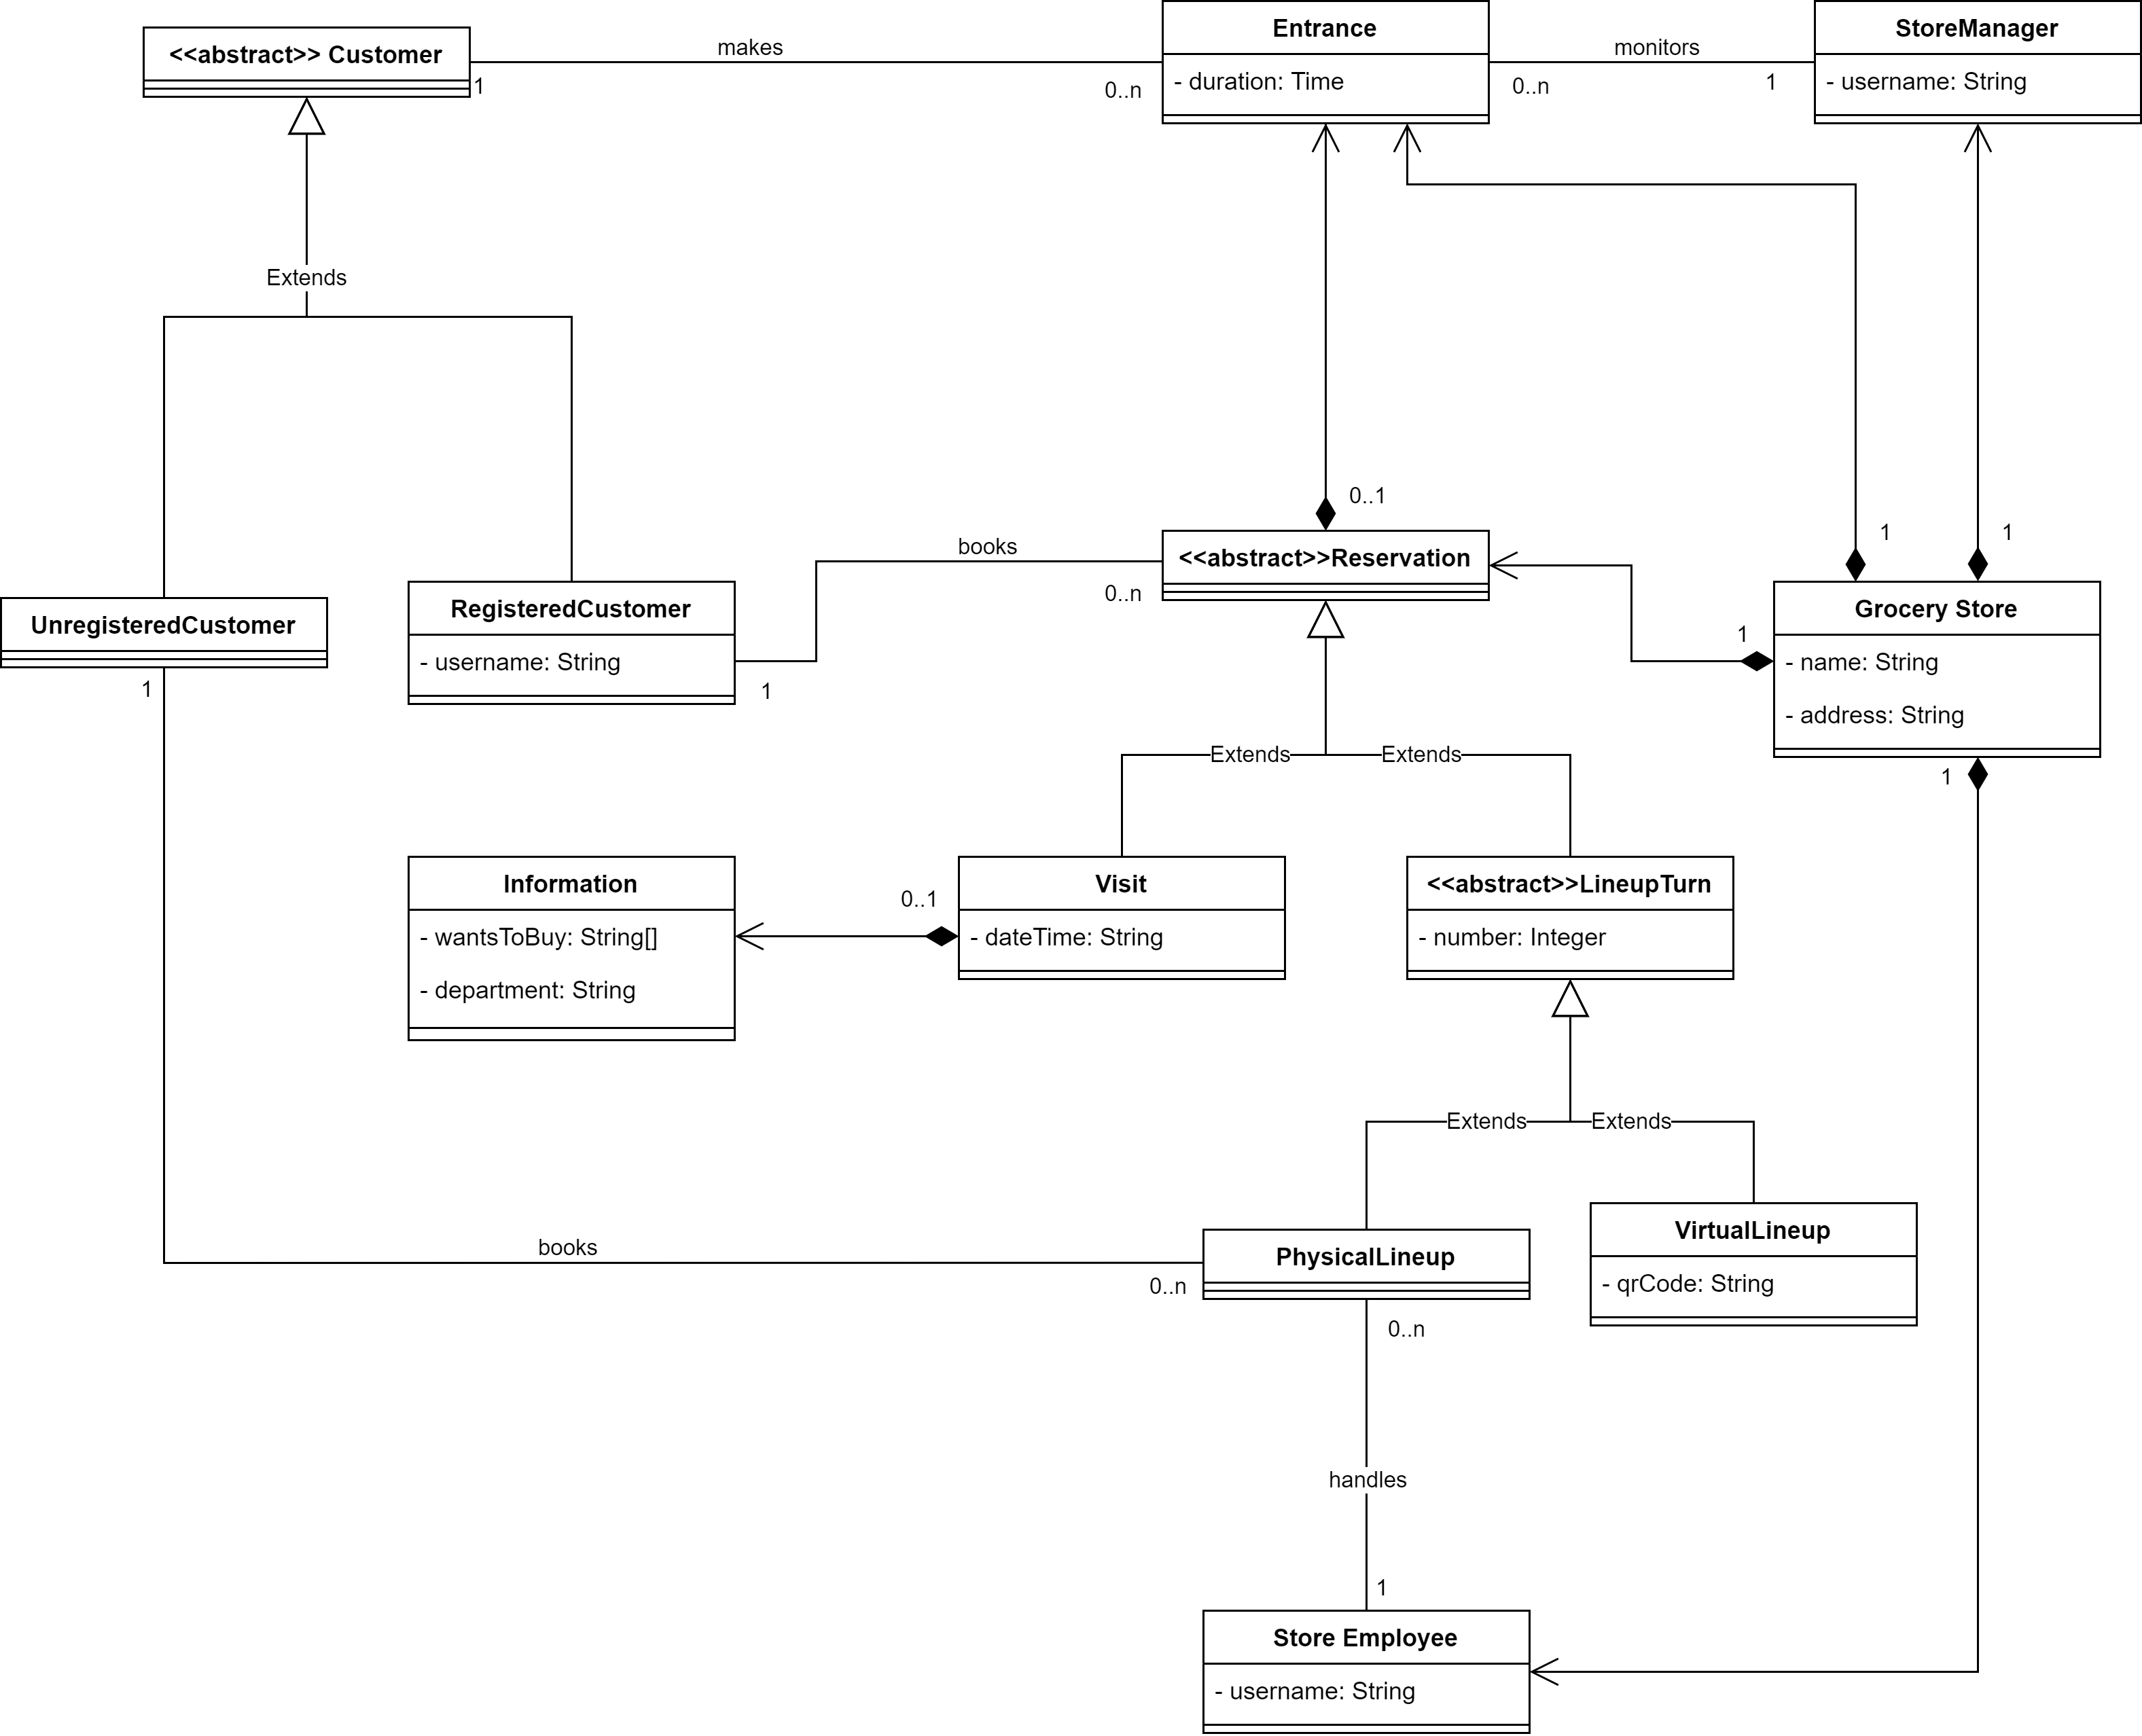
\includegraphics[width=\textwidth]{class_diagram.png}


\subsection{Dynamic Class Behaviour Models}
The below state diagrams shows some	critical aspects of	the	application, how the behaviour of these critical aspects is modeled and the evolution of their states.

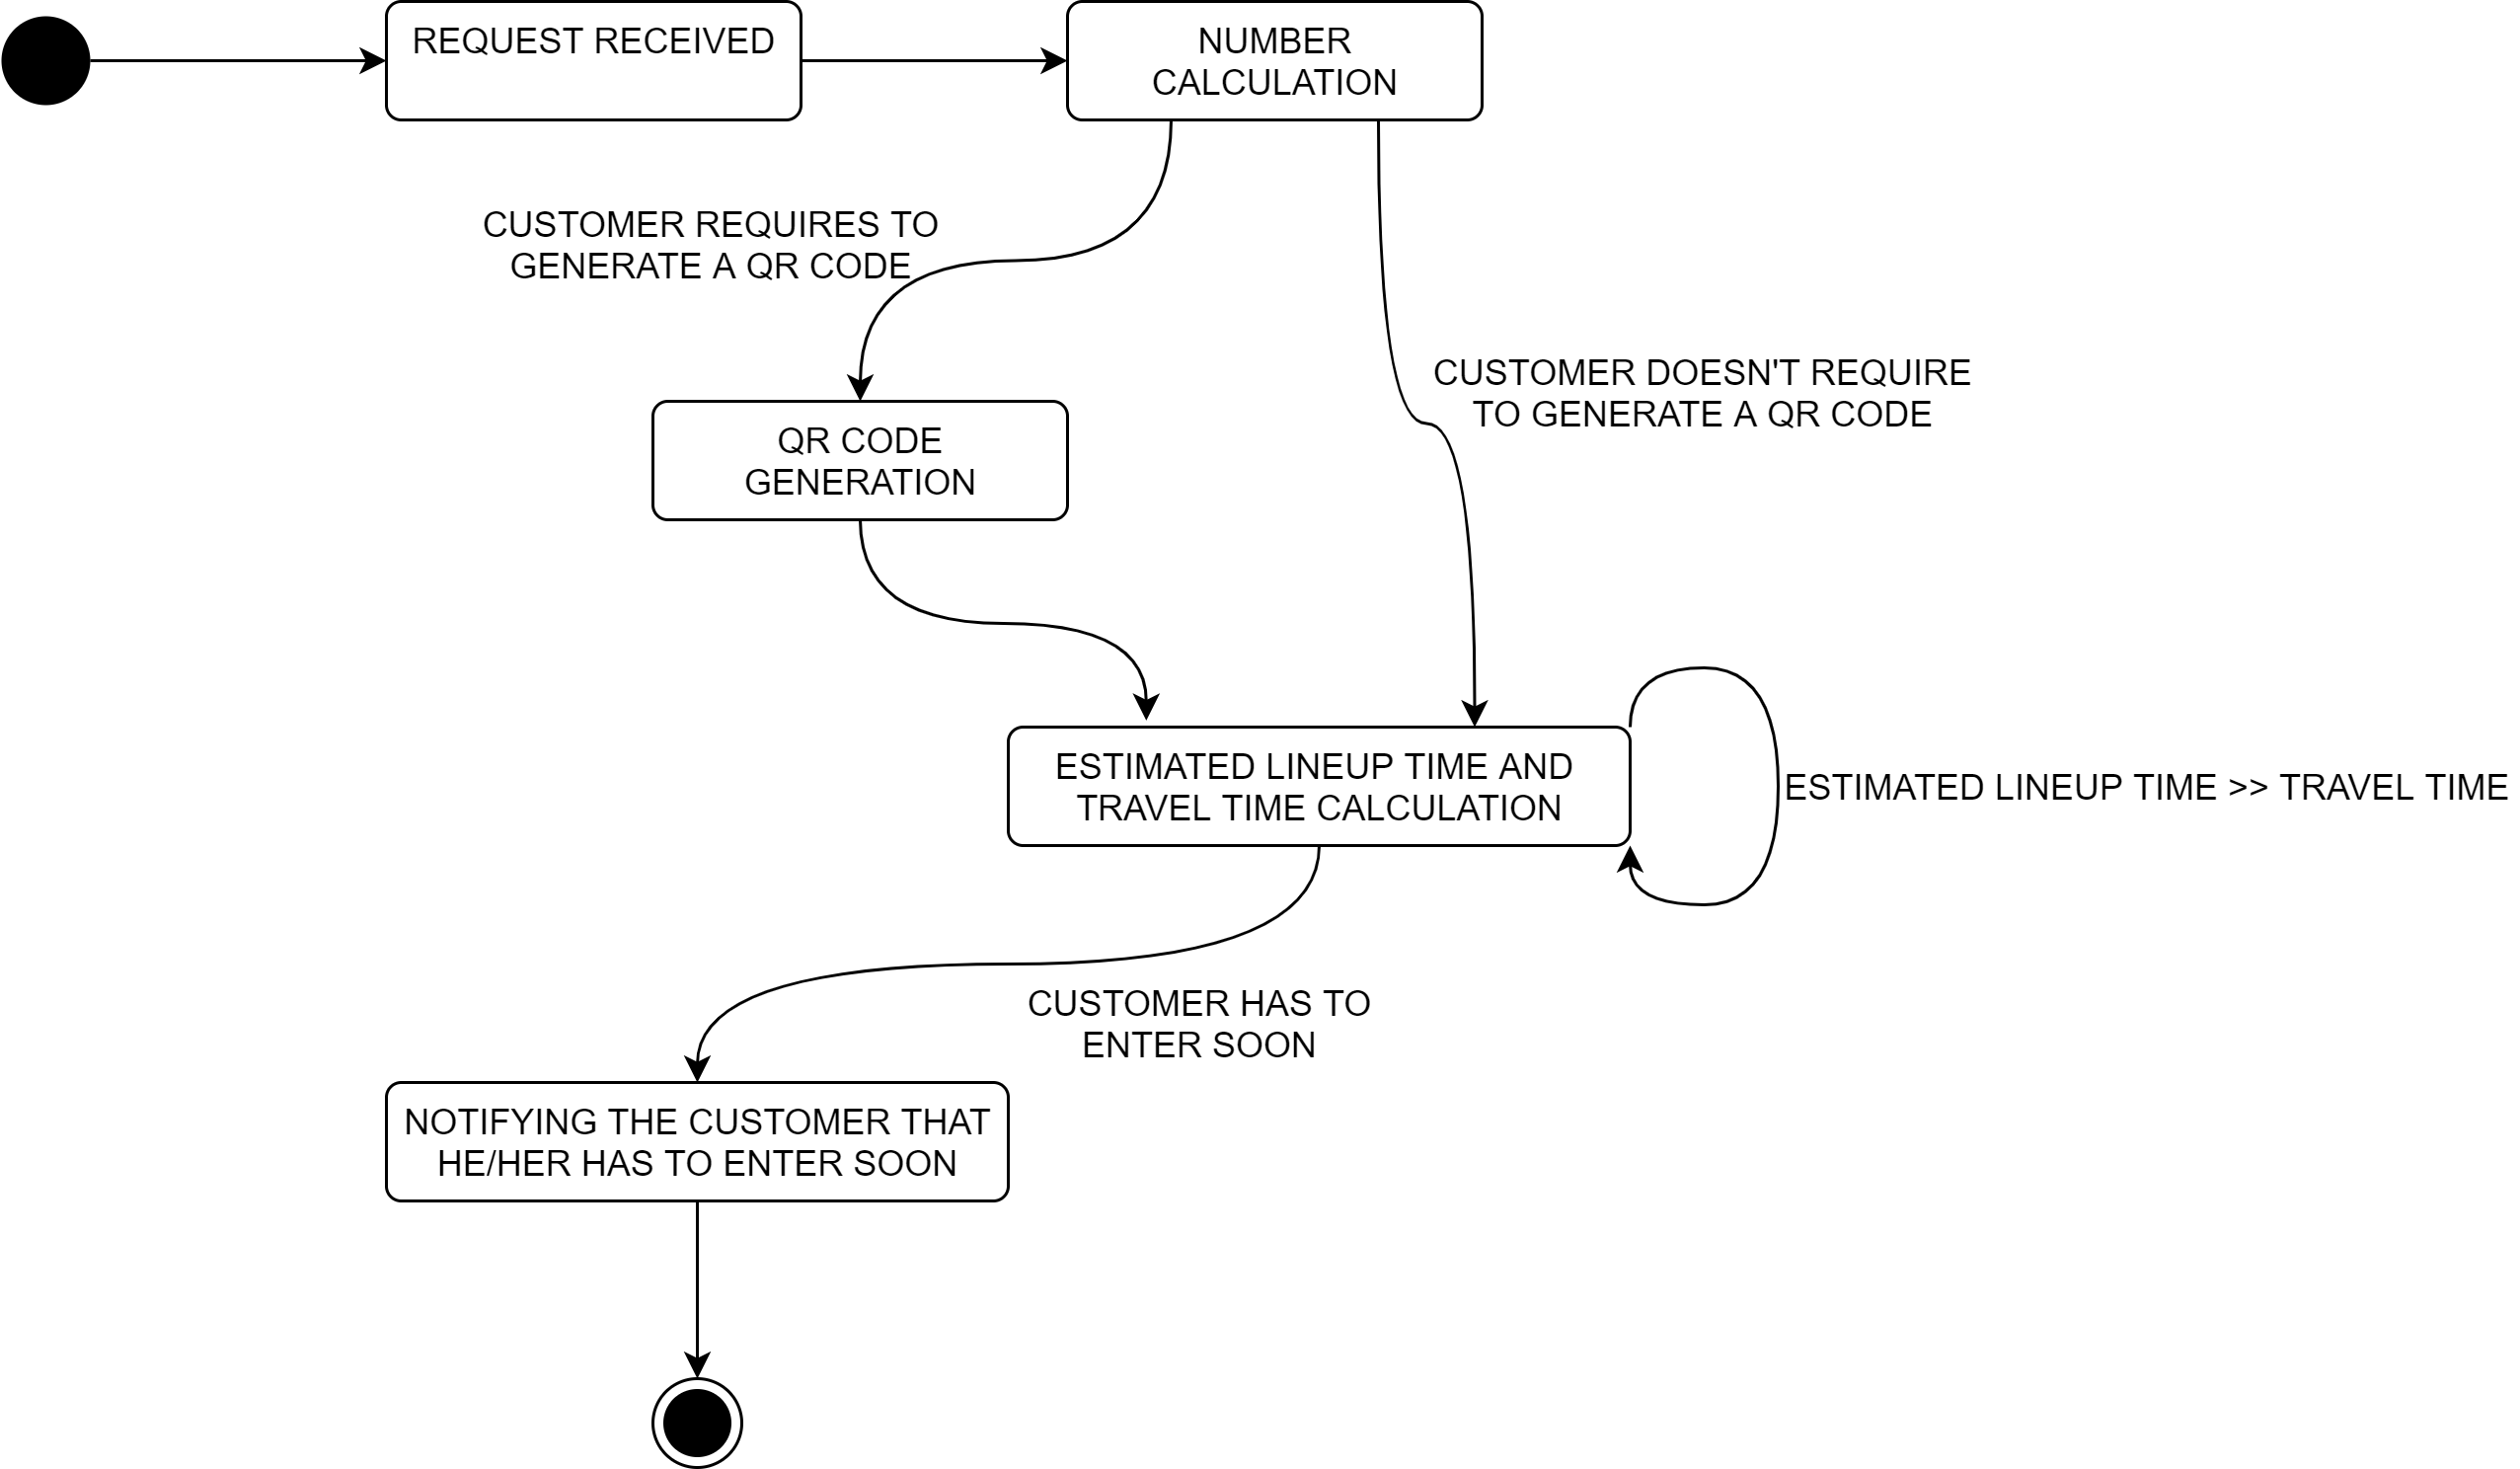
\includegraphics[width=\textwidth]{state_diagram1.png}

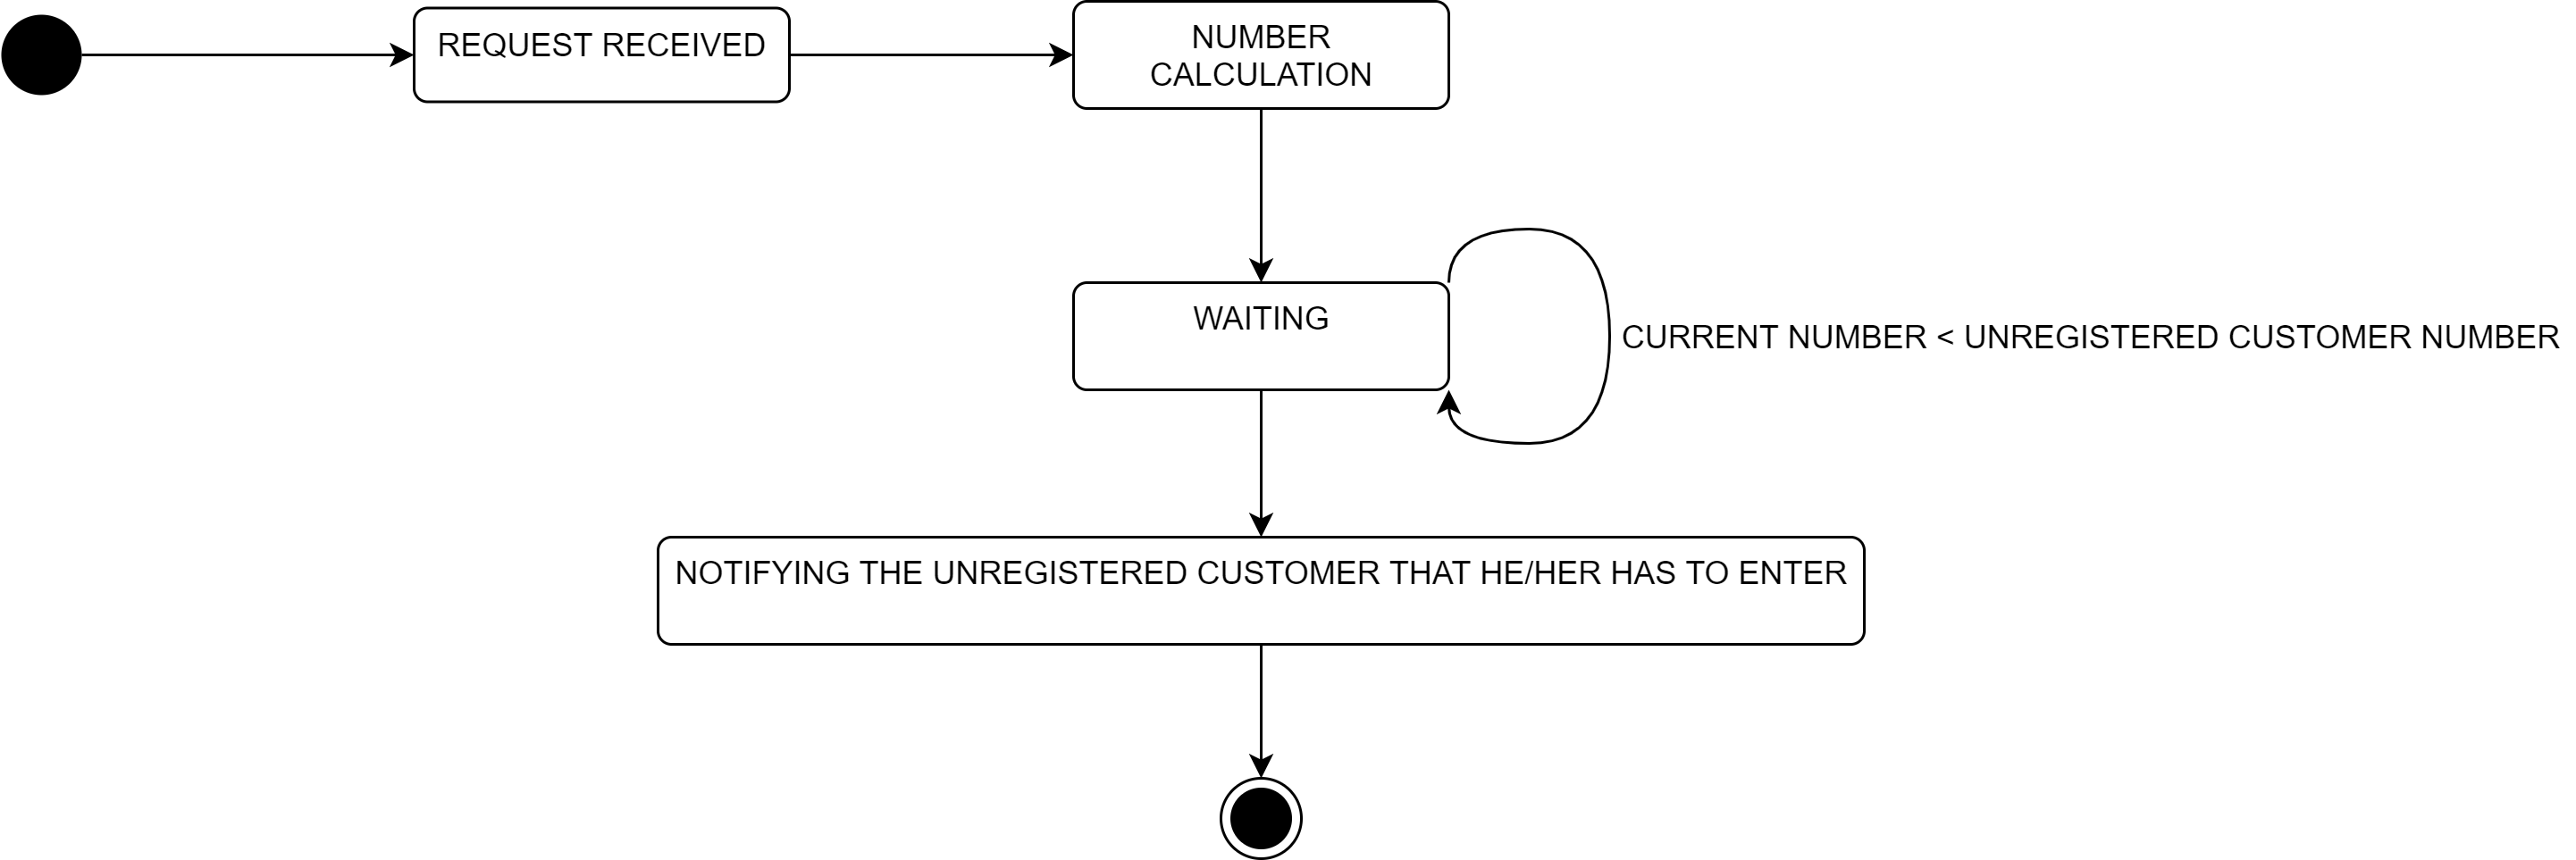
\includegraphics[width=\textwidth]{state_diagram2.png}

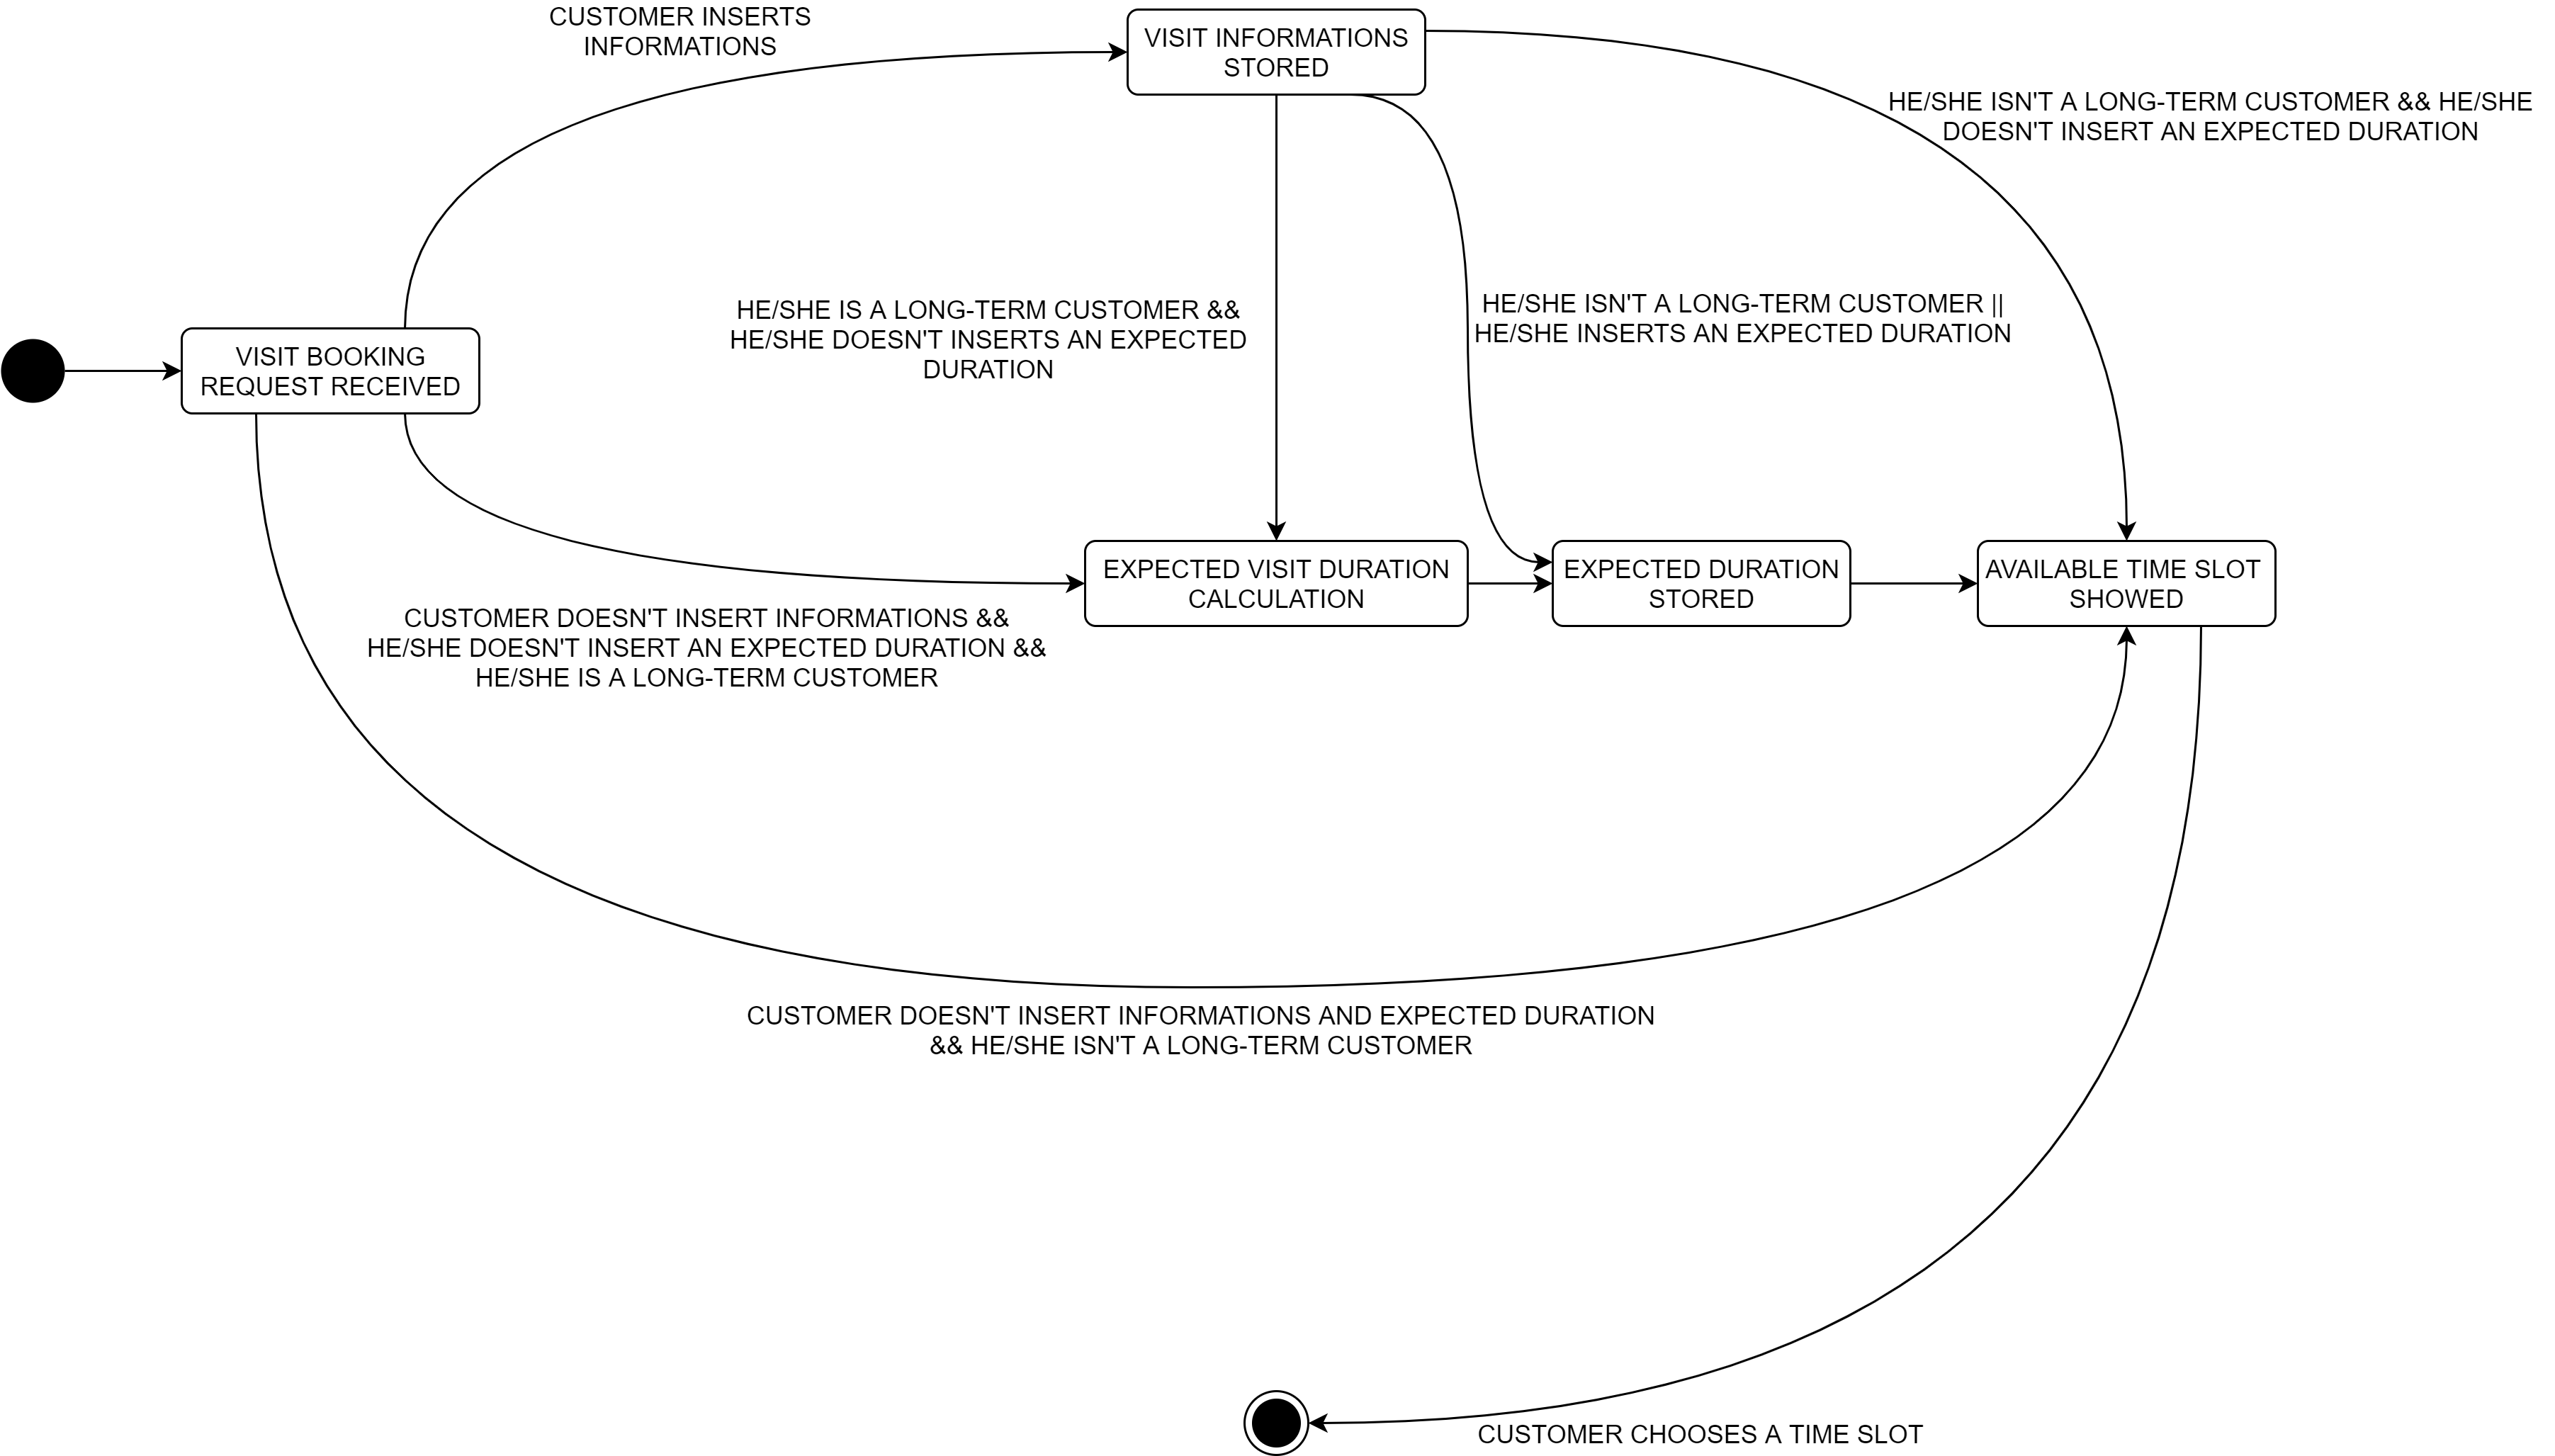
\includegraphics[width=\textwidth]{state_diagram3.png}

	\section{Product functions}

		Here is the description of the major function that CLup system has. In particular, we identified four significative function, they are :
\begin{itemize}
    \item \textbf{Reservation of a number for a line up :}
    \item \textbf{Booking a visit :}
    \item \textbf{Identification of a customer at the store entrance :}
    \item \textbf{Collection and data elaboration :}
\end{itemize}

	\section{User characteristics}

		The actors of the application are the following:
\begin{itemize}
    \item \textbf{Unregistered customer:} a person who can sign up to the CLup service. If the user doesn't have a compatible device to register to CLup he/she can go to the store and line up there.
    \item \textbf{Registered customer:} a person passed through the registration process. He/she is able to line up digitally or to book a visit right from the CLup application.
    \item \textbf{Store employee:} a person who works at a grocery store and is registered to CLup as employee. He/she can line up customers who arrived at the store without lining up digitally. He/she will then call the customers when it's time to enter the supermarket.
    \item \textbf{Store manager:} a person who works at a grocery store as the manager of that shop. He/she can manage the store informations on the CLup platform like the opening hours or the store capacity.
\end{itemize}

	\section{Assumption, dependencies and constraints}
	
		In the specification document presented by the client we found some points that lacked in precision. In order to better clarify and to make you understand better the content of this document we decided to introduce those assumptions.
\subsection{Text assumptions}
\begin{itemize}
    \item Entrances monitoring is referred to customers using their personal QR code.
    \item QR Code scanning is not mandatory: customers who will scan their QR code when entering the store will contribute to entrances monitoring, thoose who will not will not contribute to such statistics.
    \item Previous visits durations are inserted in the CLup system in some way.
\end{itemize}

\subsection{Domain assumptions}

    \begin{center}
        {\renewcommand{\arraystretch}{2}%
        \begin{tabular}{L{2cm}L{12cm}}
            \hline
            \textbf{D1} & The CLup system is enabled only when entrances control is needed \\
            \hline
            \textbf{D2} & Store has a capacity greater than 0 \\
            \hline
            \textbf{D3} & Customer who lines up has a GPS enabled device \\
            \hline
            \textbf{D4} & GPS is enabled between the line up and the departure to approach the store \\
            \hline
            \textbf{D5} & The user has a working internet connection \\
            \hline
            \textbf{D6} & The store has an available employee to serve customers who physically want to line up and retrieve a number \\
            \hline
            \textbf{D7} & The store employee who lines up customers will call them when they are allowed to enter the store \\
            \hline
            \textbf{D8} & Stores are uniquely identified \\
            \hline
            \textbf{D9} & The customer's device, the store and the CLup system have a syncronized date and time \\
            \hline
            \textbf{D10} & A QR code scanner will be available entering the store \\
            \hline
            \textbf{D11} & The store is physically accessible \\
            \hline
            \textbf{D12} & There is a route from the customer to the store \\
            \hline
            \textbf{D13} & The estimated time to enter the store is greater than the estimated time to approach the store \\
            \hline
            \textbf{D14} & The customer stay at the store is limited in time \\
            \hline
            \textbf{D15} & No two customers have the same number when entering at the same time \\
            \hline
            \textbf{D16} & The customer who specifies what he/she will buy/what departments he/she will go to will comply with his/her estimations \\
            \hline
            \textbf{D17} & Customer has a CLup compatible device \\
            \hline
            \textbf{D18} & Store has a CLup compatible device \\
            \hline
        \end{tabular}}
    \end{center}

\chapter{Specific Requirements}\label{chapt:sum}

	\section{External Interface Requirements}

		\subsection{User Interfaces}
The application in use by the customer will let the user line up, book a visit, and view the details about the queue or the booked visit.
The web application in use by the store manager will let him view store information and statistics. The employee will use the web application to line up on behalf of visitors, to call them, to check entrances, and report exits. Functional requirements are fully described in the next subsection. 

The following mockups represent a basic idea of what the mobile app and the web app will look like.

\subsection{Hardware Interfaces}
\label{hardware interfaces}
The CLup applications interact with three types of actors and two of them share the same hardware requirements:
\begin{itemize}
    \item Regarding the customer: he/she needs an iOS/Android smartphone with a working Internet connection and GPS sensor. The application will not require a lot of computational power, therefore any recent (last couple of years) smartphone will be suitable.
    \item Regarding the store manager and the employees: he/she needs a modern web browser and an Internet connection. The web application will run easily on any desktop computer of the last decade.
\end{itemize}

\subsection{Software Interfaces}
The system will use the following external software interfaces:
\begin{itemize}
    \item \textbf{Public geodata provider:} the system will connect to a public geodata service API (like Google Maps or OpenStreetMap and the like) to compute a route from the user's location to the grocery store and in particular to retrieve an estimated travel time
    \item \textbf{Android/iOS system APIs:} the mobile application will be developed for iOS and Android, therefore it will interact with the underlying system's primitives.
\end{itemize}

\subsection{Communication Interfaces}
The mobile application and the web application will communicate with CLup via an internet connection.

	\section{Functional Requirements}

		\subsection{List of requirements}
    \begin{center}
        {\renewcommand{\arraystretch}{2}
        \begin{longtable}{L{2cm}L{12cm}}
            \hline
            \textbf{R1} & Visitors are allowed to register as customers through the CLup application \\
            \hline
            \textbf{R2} & The store manager is allowed to register as store manager through the CLup web app \\
            \hline
            \textbf{R3} & Customers are allowed to log in inside the application \\
            \hline
            \textbf{R4} & The store manager and the employee are allowed to login in inside the web application \\
            \hline
            \textbf{R5} & The store manager can insert and edit store information \\
            \hline
            \textbf{R6} & The store manager can create and edit the employees' accounts associated to his/her store \\
            \hline
            \textbf{R7} & The employee can line up a visitor who asked for that and can give him/her the number associated with the position in the queue \\
            \hline
            \textbf{R8} & The employee can report the entrance related to a line up number or a visit and the exit of each person from the store \\
            \hline
            \textbf{R9} & The line up numbers and the visits are invalidated after a period of time if not used to enter the store \\
            \hline
            \textbf{R10} & The employee can see the line up numbers/visits that are allowed to enter the store \\
            \hline
            \textbf{R11} & The CLup system notifies the employee when it's time to call a visitor who previously asked to line up at the entry point \\
            \hline
            \textbf{R12} & The store manager can see charts and analysis related to entrances made with the QR code \\
            \hline
            \textbf{R13} & Customer can generate a QR code to enter the store \\
            \hline
            \textbf{R14} & The CLup system can acquire the scanned QR code \\
            \hline
            \textbf{R15} & The CLup application has a section to line up \\
            \hline
            \textbf{R16} & The CLup application shows the estimated queue waiting time, the queue size, the estimated travel time and the number related to the position in the queue \\
            \hline
            \textbf{R17} & The application monitors the customer's position and computes the estimated travel time \\
            \hline
            \textbf{R18} & The application notifies the customer when the estimated queue waiting time is near the estimated travel time \\
            \hline
            \textbf{R19} & The system generates a unique (in an appropriate time interval) number to identify the position in the queue \\
            \hline
            \textbf{R20} & The system pushes forward the queue based on the reported exits and the scheduled visits \\
            \hline
            \textbf{R21} & The CLup application has a section to book a visit \\
            \hline
            \textbf{R22} & The CLup application shows available time slots for visits \\
            \hline
            \textbf{R23} & The system schedules visits based on related details \\
            \hline
            \textbf{R24} & The customer can insert additional details like what he/she is going to buy, the estimated visit duration or what departments he/she will go to) \\
            \hline
            \textbf{R25} & The CLup system can compute the estimated visit duration for long term customers based on previous visits \\
            \hline
        \end{longtable}}
    \end{center}

\subsection{Mapping}
    \begin{center}
        {\renewcommand{\arraystretch}{2}
        \begin{longtable}{L{2cm}L{6cm}L{6cm}}
            \hline
            \textbf{Goal} & \textbf{Requirements} & \textbf{Domain assumptions} \\
            \hline
            \textbf{G1} & R1, R2, R3, R4, R6 & D5, D18, D19 \\
            \hline
            \textbf{G2} & R3, R4, R6, R8, R9, R11, R17, R18, R19, R20 & D1, D3, D4, D5, D7, D8, D10, D14, D15, D18, D19 \\
            \hline
            \textbf{G3} & R3, R4, R6, R8, R10, R14 & D3, D7, D11, D12, D13, D16, D18, D19 \\
            \hline
            \textbf{G4} & R4, R6, R7 & D2, D3, D6, D12, D13 \\
            \hline
            \textbf{G5} & R4, R5, R6, R7, R8, R10, R15, R20, R21, R23 & D1, D2, D5, D6, D7, D15, D17, D18, D19 \\
            \hline
            \textbf{G6} & R4, R6, R7, R9, R11 & D1, D2, D3, D5, D6, D8, D10, D15, D18, D19 \\
            \hline
            \textbf{G7} & R3, R21, R22, R24 & D1, D3, D5, D9, D10, D13, 18 \\
            \hline
            \textbf{G8} & R3, R13, R15, R16, R19 & D1, D2, D3, D5, D9, D10, D13, D18 \\
            \hline
            \textbf{G9} & R4, R5, R12, R14 & D1, D5, D11, D18, D19 \\
            \hline
            \textbf{G10} & R3, R16, R17, R18 & D4, D5, D10, D12, D13, D14, D18 \\
            \hline
        \end{longtable}}

        {\renewcommand{\arraystretch}{1.5}
        \begin{longtable}{L{2cm}L{12cm}}
            \hline
            \rowcolor{shadeColorGoal}\textbf{G1} & \textbf{Everyone can use and interact with the CLup system accordingly with itsfeatures and processes} \\
            \hline
            \rowcolor{shadeColorRequirement} R1 & Visitors are allowed to register as customers through the CLup application \\
            \hline
            \rowcolor{shadeColorRequirement} R2 & The store manager is allowed to register as store manager through the CLup web app \\
            \hline
            \rowcolor{shadeColorRequirement} R3 & Customers are allowed to log in inside the application \\
            \hline
            \rowcolor{shadeColorRequirement} R4 & The store manager and the employee are allowed to login in inside the web application \\
            \hline
            \rowcolor{shadeColorRequirement} R6 & The store manager can create and edit the employees’ accounts associated to his/her store \\
            \hline
            \rowcolor{shadeColorDomainAssumption} D5 & The user has a working internet connection \\
            \hline
            \rowcolor{shadeColorDomainAssumption} D18 & Customer who wants to directly interact with the CLup system has a compatible device \\
            \hline
            \rowcolor{shadeColorDomainAssumption} D19 & Store has a CLup compatible device \\
            \hline
        \end{longtable}}

        {\renewcommand{\arraystretch}{1.5}
        \begin{longtable}{L{2cm}L{12cm}}
            \hline
            \rowcolor{shadeColorGoal}\textbf{G2} & \textbf{All customers who reserve a place in the queue will be called} \\
            \hline
            \rowcolor{shadeColorRequirement} R3 & Customers are allowed to log in inside the application \\
            \hline
            \rowcolor{shadeColorRequirement} R4 & The store manager and the employee are allowed to login in inside the web application \\
            \hline
            \rowcolor{shadeColorRequirement} R6 & The store manager can create and edit the employees’ accounts associated to his/her store \\
            \hline
            \rowcolor{shadeColorRequirement} R8 & The employee can report the entrance related to a line up number or a visit and the exit of each person from the store \\
            \hline
            \rowcolor{shadeColorRequirement} R9 & The line up numbers and the visits are invalidated after a period of time if not used to enter the store \\
            \hline
            \rowcolor{shadeColorRequirement} R11 & The CLup system notifies the employee when it’s time to call a visitor who previously asked to line up at the entry point \\
            \hline
            \rowcolor{shadeColorRequirement} R17 & The application monitors the customer’s position and computes the estimated travel time \\
            \hline
            \rowcolor{shadeColorRequirement} R18 & The application notifies the customer when the estimated queue waiting time is near the estimated travel time \\
            \hline
            \rowcolor{shadeColorRequirement} R19 & The system generates a unique (in an appropriate time interval) number to identify the position in the queue \\
            \hline
            \rowcolor{shadeColorRequirement} R20 & The system pushes forward the queue based on the reported exits and the scheduled visits \\
            \hline
            \rowcolor{shadeColorDomainAssumption} D1 & All customers use CLup to access the store \\
            \hline
            \rowcolor{shadeColorDomainAssumption} D3 & Store has a capacity greater than 0 \\
            \hline
            \rowcolor{shadeColorDomainAssumption} D4 & GPS is enabled between the line up request and the departure to approach the store \\
            \hline
            \rowcolor{shadeColorDomainAssumption} D5 & The user has a working internet connection \\
            \hline
            \rowcolor{shadeColorDomainAssumption} D7 & The store has an available employee to check for entrances and to report exits \\
            \hline
            \rowcolor{shadeColorDomainAssumption} D8 & The store employee who lines up customers will call them when they are allowed to enter the store \\
            \hline
            \rowcolor{shadeColorDomainAssumption} D10 & The customer’s device, the store and the CLup system have a syncronized date and time \\
            \hline
            \rowcolor{shadeColorDomainAssumption} D14 & The estimated time to enter the store is greater than the estimated time to approach the store \\
            \hline
            \rowcolor{shadeColorDomainAssumption} D15 & The customer stay at the store is limited in time \\
            \hline
            \rowcolor{shadeColorDomainAssumption} D18 & Customer who wants to directly interact with the CLup system has a compatible device \\
            \hline
            \rowcolor{shadeColorDomainAssumption} D19 & Store has a CLup compatible device \\
            \hline
        \end{longtable}}

        {\renewcommand{\arraystretch}{1.5}
        \begin{longtable}{L{2cm}L{12cm}}
            \hline
            \rowcolor{shadeColorGoal}\textbf{G3} & \textbf{Allow customers to enter the store once their number has been called or ifthey have booked a visit for that time slot} \\
            \hline
            \rowcolor{shadeColorRequirement} R3 & Customers are allowed to log in inside the application \\
            \hline
            \rowcolor{shadeColorRequirement} R4 & The store manager and the employee are allowed to login in inside the web application \\
            \hline
            \rowcolor{shadeColorRequirement} R6 & The store manager can create and edit the employees’ accounts associated to his/her store \\
            \hline
            \rowcolor{shadeColorRequirement} R8 & The employee can report the entrance related to a line up number or a visit and the exit of each person from the store \\
            \hline
            \rowcolor{shadeColorRequirement} R10 & The employee can see the line up numbers/visits that are allowed to enter the store \\
            \hline
            \rowcolor{shadeColorRequirement} R14 & The CLup system can acquire the scanned QR code \\
            \hline
            \rowcolor{shadeColorDomainAssumption} D3 & Store has a capacity greater than 0 \\
            \hline
            \rowcolor{shadeColorDomainAssumption} D7 & The store has an available employee to check for entrances and to report exits \\
            \hline
            \rowcolor{shadeColorDomainAssumption} D11 & A QR code scanner will be available entering the store \\
            \hline
            \rowcolor{shadeColorDomainAssumption} D12 & The store is physically accessible \\
            \hline
            \rowcolor{shadeColorDomainAssumption} D13 & There is a route from the customer to the store \\
            \hline
            \rowcolor{shadeColorDomainAssumption} D16 & No two customers have the same number when entering at the same time \\
            \hline
            \rowcolor{shadeColorDomainAssumption} D18 & Customer who wants to directly interact with the CLup system has a compatible device \\
            \hline
            \rowcolor{shadeColorDomainAssumption} D19 & Store has a CLup compatible device \\
            \hline
        \end{longtable}}

        {\renewcommand{\arraystretch}{1.5}
        \begin{longtable}{L{2cm}L{12cm}}
            \hline
            \rowcolor{shadeColorGoal}\textbf{G4} & \textbf{Customers who go to the supermarket without a number/booking are allowedto line up at the store} \\
            \hline
            \rowcolor{shadeColorRequirement} R4 & The store manager and the employee are allowed to login in inside the web application \\
            \hline
            \rowcolor{shadeColorRequirement} R6 & The store manager can create and edit the employees’ accounts associated to his/her store \\
            \hline
            \rowcolor{shadeColorRequirement} R7 & The employee can line up a visitor who asked for that and can give him/her the number associated with the position in the queue \\
            \hline
            \rowcolor{shadeColorDomainAssumption} D2 & The CLup line up system is enabled only when entrances control is needed \\
            \hline
            \rowcolor{shadeColorDomainAssumption} D3 & Store has a capacity greater than 0 \\
            \hline
            \rowcolor{shadeColorDomainAssumption} D6 & The store has an available employee to serve customers who physically want to line up and retrieve a number \\
            \hline
            \rowcolor{shadeColorDomainAssumption} D12 & The store is physically accessible \\
            \hline
            \rowcolor{shadeColorDomainAssumption} D13 & There is a route from the customer to the store \\
            \hline
        \end{longtable}}

        {\renewcommand{\arraystretch}{1.5}
        \begin{longtable}{L{2cm}L{12cm}}
            \hline
            \rowcolor{shadeColorGoal}\textbf{G5} & \textbf{Inside the grocery store it must be feasible to follow Covid19 regulations} \\
            \hline
            \rowcolor{shadeColorRequirement} R4 & The store manager and the employee are allowed to login in inside the web application \\
            \hline
            \rowcolor{shadeColorRequirement} R5 & The store manager can insert and edit store information \\
            \hline
            \rowcolor{shadeColorRequirement} R6 & The store manager can create and edit the employees’ accounts associated to his/her store \\
            \hline
            \rowcolor{shadeColorRequirement} R7 & The employee can line up a visitor who asked for that and can give him/her the number associated with the position in the queue \\
            \hline
            \rowcolor{shadeColorRequirement} R8 & The employee can report the entrance related to a line up number or a visit and the exit of each person from the store \\
            \hline
            \rowcolor{shadeColorRequirement} R10 & The employee can see the line up numbers/visits that are allowed to enter the store \\
            \hline
            \rowcolor{shadeColorRequirement} R15 & The CLup application has a section to line up \\
            \hline
            \rowcolor{shadeColorRequirement} R20 & The system pushes forward the queue based on the reported exits and the scheduled visits \\
            \hline
            \rowcolor{shadeColorRequirement} R21 & The CLup application has a section to book a visit \\
            \hline
            \rowcolor{shadeColorRequirement} R23 & The system schedules visits based on related details \\
            \hline
            \rowcolor{shadeColorDomainAssumption} D1 & All customers use CLup to access the store \\
            \hline
            \rowcolor{shadeColorDomainAssumption} D2 & The CLup line up system is enabled only when entrances control is needed \\
            \hline
            \rowcolor{shadeColorDomainAssumption} D5 & The user has a working internet connection \\
            \hline
            \rowcolor{shadeColorDomainAssumption} D6 & The store has an available employee to serve customers who physically want to line up and retrieve a number \\
            \hline
            \rowcolor{shadeColorDomainAssumption} D7 & The store has an available employee to check for entrances and to report exits \\
            \hline
            \rowcolor{shadeColorDomainAssumption} D15 & The customer stay at the store is limited in time \\
            \hline
            \rowcolor{shadeColorDomainAssumption} D17 & The customer who specifies what he/she will buy/what departments he/she will go to will comply with his/her estimations \\
            \hline
            \rowcolor{shadeColorDomainAssumption} D18 & Customer who wants to directly interact with the CLup system has a compatible device \\
            \hline
            \rowcolor{shadeColorDomainAssumption} D19 & Store has a CLup compatible device \\
            \hline
        \end{longtable}}

        {\renewcommand{\arraystretch}{1.5}
        \begin{longtable}{L{2cm}L{12cm}}
            \hline
            \rowcolor{shadeColorGoal}\textbf{G6} & \textbf{Outside the grocery store there must not be long queues or overcrowding} \\
            \hline
            \rowcolor{shadeColorRequirement} R4 & The store manager and the employee are allowed to login in inside the web application \\
            \hline
            \rowcolor{shadeColorRequirement} R6 & The store manager can create and edit the employees’ accounts associated to his/her store \\
            \hline
            \rowcolor{shadeColorRequirement} R7 & The employee can line up a visitor who asked for that and can give him/her the number associated with the position in the queue \\
            \hline
            \rowcolor{shadeColorRequirement} R9 & The line up numbers and the visits are invalidated after a period of time if not used to enter the store \\
            \hline
            \rowcolor{shadeColorRequirement} R11 & The CLup system notifies the employee when it’s time to call a visitor who previously asked to line up at the entry point \\
            \hline
            \rowcolor{shadeColorDomainAssumption} D1 & All customers use CLup to access the store \\
            \hline
            \rowcolor{shadeColorDomainAssumption} D2 & The CLup line up system is enabled only when entrances control is needed \\
            \hline
            \rowcolor{shadeColorDomainAssumption} D3 & Store has a capacity greater than 0 \\
            \hline
            \rowcolor{shadeColorDomainAssumption} D5 & The user has a working internet connection \\
            \hline
            \rowcolor{shadeColorDomainAssumption} D6 & The store has an available employee to serve customers who physically want to line up and retrieve a number \\
            \hline
            \rowcolor{shadeColorDomainAssumption} D8 & The store employee who lines up customers will call them when they are allowed to enter the store \\
            \hline
            \rowcolor{shadeColorDomainAssumption} D10 & The customer’s device, the store and the CLup system have a syncronized date and time \\
            \hline
            \rowcolor{shadeColorDomainAssumption} D15 & The customer stay at the store is limited in time \\
            \hline
            \rowcolor{shadeColorDomainAssumption} D18 & Customer who wants to directly interact with the CLup system has a compatible device \\
            \hline
            \rowcolor{shadeColorDomainAssumption} D19 & Store has a CLup compatible device \\
            \hline
        \end{longtable}}

        {\renewcommand{\arraystretch}{1.5}
        \begin{longtable}{L{2cm}L{12cm}}
            \hline
            \rowcolor{shadeColorGoal}\textbf{G7} & \textbf{Customer is allowed to book a visit through the CLup system} \\
            \hline
            \rowcolor{shadeColorRequirement} R3 & Customers are allowed to log in inside the application \\
            \hline
            \rowcolor{shadeColorRequirement} R21 & The CLup application has a section to book a visit \\
            \hline
            \rowcolor{shadeColorRequirement} R22 & The CLup application shows available time slots for visits \\
            \hline
            \rowcolor{shadeColorRequirement} R24 & The customer can insert additional details like what he/she is going to buy, the estimated visit duration or what departments he/she will go to) \\
            \hline
            \rowcolor{shadeColorDomainAssumption} D1 & All customers use CLup to access the store \\
            \hline
            \rowcolor{shadeColorDomainAssumption} D3 & Store has a capacity greater than 0 \\
            \hline
            \rowcolor{shadeColorDomainAssumption} D5 & The user has a working internet connection \\
            \hline
            \rowcolor{shadeColorDomainAssumption} D9 & Stores are uniquely identified \\
            \hline
            \rowcolor{shadeColorDomainAssumption} D10 & The customer’s device, the store and the CLup system have a syncronized date and time \\
            \hline
            \rowcolor{shadeColorDomainAssumption} D13 & There is a route from the customer to the store \\
            \hline
            \rowcolor{shadeColorDomainAssumption} D18 & Customer who wants to directly interact with the CLup system has a compatible device \\
            \hline
        \end{longtable}}

        {\renewcommand{\arraystretch}{1.5}
        \begin{longtable}{L{2cm}L{12cm}}
            \hline
            \rowcolor{shadeColorGoal}\textbf{G8} & \textbf{Customer is allowed to line up through the CLup system} \\
            \hline
            \rowcolor{shadeColorRequirement} R3 & Customers are allowed to log in inside the application \\
            \hline
            \rowcolor{shadeColorRequirement} R13 & Customer can generate a QR code to enter the store \\
            \hline
            \rowcolor{shadeColorRequirement} R15 & The CLup application has a section to line up \\
            \hline
            \rowcolor{shadeColorRequirement} R16 & The CLup application shows the estimated queue waiting time, the queue size, the estimated travel time and the number related to the position in the queue \\
            \hline
            \rowcolor{shadeColorRequirement} R19 & The system generates a unique (in an appropriate time interval) number toidentify the position in the queue \\
            \hline
            \rowcolor{shadeColorDomainAssumption} D1 & All customers use CLup to access the store \\
            \hline
            \rowcolor{shadeColorDomainAssumption} D2 & The CLup line up system is enabled only when entrances control is needed \\
            \hline
            \rowcolor{shadeColorDomainAssumption} D3 & Store has a capacity greater than 0 \\
            \hline
            \rowcolor{shadeColorDomainAssumption} D5 & The user has a working internet connection \\
            \hline
            \rowcolor{shadeColorDomainAssumption} D9 & Stores are uniquely identified \\
            \hline
            \rowcolor{shadeColorDomainAssumption} D10 & The customer’s device, the store and the CLup system have a syncronized date and time \\
            \hline
            \rowcolor{shadeColorDomainAssumption} D13 & There is a route from the customer to the store \\
            \hline
            \rowcolor{shadeColorDomainAssumption} D18 & Customer who wants to directly interact with the CLup system has a compatible device \\
            \hline
        \end{longtable}}

        {\renewcommand{\arraystretch}{1.5}
        \begin{longtable}{L{2cm}L{12cm}}
            \hline
            \rowcolor{shadeColorGoal}\textbf{G9} & \textbf{The store manager is allowed to monitor entrances of customers that used theQR Code} \\
            \hline
            \rowcolor{shadeColorRequirement} R4 & The store manager and the employee are allowed to login in inside the web application \\
            \hline
            \rowcolor{shadeColorRequirement} R5 & The store manager can insert and edit store information \\
            \hline
            \rowcolor{shadeColorRequirement} R12 & The store manager can see charts and analysis related to entrances made with the QR code \\
            \hline
            \rowcolor{shadeColorRequirement} R14 & The CLup system can acquire the scanned QR code \\
            \hline
            \rowcolor{shadeColorDomainAssumption} D1 & All customers use CLup to access the store \\
            \hline
            \rowcolor{shadeColorDomainAssumption} D5 & The user has a working internet connection \\
            \hline
            \rowcolor{shadeColorDomainAssumption} D11 & A QR code scanner will be available entering the store \\
            \hline
            \rowcolor{shadeColorDomainAssumption} D18 & Customer who wants to directly interact with the CLup system has a compatible device \\
            \hline
            \rowcolor{shadeColorDomainAssumption} D19 & Store has a CLup compatible device \\
            \hline
        \end{longtable}}

        {\renewcommand{\arraystretch}{1.5}
        \begin{longtable}{L{2cm}L{12cm}}
            \hline
            \rowcolor{shadeColorGoal}\textbf{G10} & \textbf{Customer is allowed to approach the store in time with respect to his positionin the queue} \\
            \hline
            \rowcolor{shadeColorRequirement} R3 & Customers are allowed to log in inside the application \\
            \hline
            \rowcolor{shadeColorRequirement} R16 & The CLup application shows the estimated queue waiting time, the queue size, the estimated travel time and the number related to the position in the queue \\
            \hline
            \rowcolor{shadeColorRequirement} R17 & The application monitors the customer’s position and computes the estimated travel time \\
            \hline
            \rowcolor{shadeColorRequirement} R18 & The application notifies the customer when the estimated queue waiting time is near the estimated travel time \\
            \hline
            \rowcolor{shadeColorDomainAssumption} D4 & GPS is enabled between the line up request and the departure to approach the store \\
            \hline
            \rowcolor{shadeColorDomainAssumption} D5 & The user has a working internet connection \\
            \hline
            \rowcolor{shadeColorDomainAssumption} D10 & The customer’s device, the store and the CLup system have a syncronized date and time \\
            \hline
            \rowcolor{shadeColorDomainAssumption} D12 & The store is physically accessible \\
            \hline
            \rowcolor{shadeColorDomainAssumption} D13 & There is a route from the customer to the store \\
            \hline
            \rowcolor{shadeColorDomainAssumption} D14 & The estimated time to enter the store is greater than the estimated time to approach the store \\
            \hline
            \rowcolor{shadeColorDomainAssumption} D18 & Customer who wants to directly interact with the CLup system has a compatible device \\
            \hline
        \end{longtable}}
    \end{center}

\subsection{Use Cases}

    In this section we presents some use cases of CLup System. Use cases diagram is first illustrated to give a general and abstract view of the actors and use cases associated with them (\textit{Section 3.2.3.1}). After that, all use cases illustrated in the diagram are described in their particular (\textit{Section 3.2.3.2}).
    \subsubsection{Use Cases Diagrams}
    To facilitate the readability of the diagram, it is divided into 4 diagrams, each dedicated to a single actor.
        \begin{center}

            \includegraphics*[width = \textwidth]{visitor_use_cases_diagram.png}

            \includegraphics*[width = \textwidth]{customer_use_cases_diagram.png}

            \includegraphics*[width = \textwidth]{store_employee_use_cases_diagram.png}

            \includegraphics*[width = \textwidth]{store_manager_use_cases_diagram.png}
            
        \end{center}

    \subsubsection{Use Cases Description}
        \begin{enumerate}
            \item \textbf{Registration to CLup as Customer}{\renewcommand{\arraystretch}{2}
            \begin{longtable}{|L{4cm}|L{10cm}|}
                \hline
                \textbf{Name} & Registration to CLup as a Customer \\
                \hline
                \textbf{Actors} & Visitor \\
                \hline
                \textbf{Entry Condition} & / \\
                \hline
                \textbf{Event Flow} & The Event Flow is: \begin{enumerate}
                        \item The Visitor opens the CLup application
                        \item The Visitor clicks on the "Sign up" button
                        \item The Visitor fills in all the mandatory fields
                        \item The Visitor clicks on the "Confirm" button
                        \item The System stores the information about the Visitor
                    \end{enumerate} \\
                \hline
                \textbf{Exit Condition} & The Visitor is registered and he/she is now a Customer. \\
                \hline
                \textbf{Exception} & The Exceptions are: \begin{enumerate}
                        \item The Visitor chooses an email or a username already used by another Customer
                        \item The Visitor inserts invalid information
                    \end{enumerate} Both the exceptions listed above are notified and the Visitor is returned to step (c)  \\
                \hline
                \textbf{Special Requirements} & / \\
                \hline
            \end{longtable}}
            \item \textbf{Registration to CLup as Store Manager}{\renewcommand{\arraystretch}{2}
            \begin{longtable}{|L{4cm}|L{10cm}|}
                \hline
                \textbf{Name} & Registration to CLup as Store Manager \\
                \hline
                \textbf{Actors} & Visitor \\
                \hline
                \textbf{Entry Condition} & / \\
                \hline
                \textbf{Event Flow} & The Event Flow is: \begin{enumerate}
                        \item The Visitor opens the CLup web app
                        \item The Visitor clicks on the "Sign up and register your activity" button
                        \item The Visitor fills in all the mandatory fields on himself/herself
                        \item The Visitor fills in all the mandatory fields on the Store and he/she clicks on the "Next" button
                        \item The Visitor sign up all the Store Employees that will be able to interact with the system
                        \item The Visitor clicks on the "Confirm" button
                        \item The System stores the information about the Visitor, the Store and the Store Employees
                    \end{enumerate} \\
                \hline
                \textbf{Exit Condition} & The Visitor is registered and he/she is now a Store Manager. The system has saved all store information and Store Employees accounts have been registered. \\
                \hline
                \textbf{Exception} & The Exceptions are: \begin{enumerate}
                        \item The Visitor chooses an email or a username already used by another Customer
                        \item The Visitor inserts invalid information
                    \end{enumerate} The exceptions listed above are notified and the Visitor is returned to step where error occurred: (c) or (d) or (e) \\
                \hline
                \textbf{Special Requirements} & / \\
                \hline
            \end{longtable}}
            \item \textbf{Login to the application}{\renewcommand{\arraystretch}{2}
            \begin{longtable}{|L{4cm}|L{10cm}|}
                \hline
                \textbf{Name} & Login to the application \\
                \hline
                \textbf{Actors} & Customer \\
                \hline
                \textbf{Entry Condition} & / \\
                \hline
                \textbf{Event Flow} & The Event Flow is: \begin{enumerate}
                        \item The Customer opens the CLup application
                        \item The Customer clicks on the "Login" button
                        \item The Customer inserts his/her username and password
                        \item The Customer clicks on the "Confirm" button
                    \end{enumerate} \\
                \hline
                \textbf{Exit Condition} & The Customer is logged. \\
                \hline
                \textbf{Exception} & The Exceptions are: \begin{enumerate}
                        \item The Customer inserts wrong username and/or password
                    \end{enumerate} The exception listed above is notified and the Customer is returned to step (c) \\
                \hline
                \textbf{Special Requirements} & / \\
                \hline
            \end{longtable}}
            \item \textbf{Login to the web app}{\renewcommand{\arraystretch}{2}
            \begin{longtable}{|L{4cm}|L{10cm}|}
                \hline
                \textbf{Name} & Login to the web app \\
                \hline
                \textbf{Actors} & Store Manager/Store Employee \\
                \hline
                \textbf{Entry Condition} & / \\
                \hline
                \textbf{Event Flow} & The Event Flow is: \begin{enumerate}
                        \item The Store Manager/Store Employee opens the CLup web app
                        \item The Store Manager/Store Employee clicks on the "Login" button
                        \item The Store Manager/Store Employee inserts his/her username and password
                        \item The Store Manager/Store Employee clicks on the "Confirm" button
                    \end{enumerate} \\
                \hline
                \textbf{Exit Condition} & The Store Manager/Store Employee is logged. \\
                \hline
                \textbf{Exception} & The Exceptions are: \begin{enumerate}
                        \item The Customer inserts wrong username and/or password
                    \end{enumerate} The exception listed above is notified and the Customer is returned to step (c) \\
                \hline
                \textbf{Special Requirements} & / \\
                \hline
            \end{longtable}}
            \item \textbf{Lining up via store}{\renewcommand{\arraystretch}{2}
            \begin{longtable}{|L{4cm}|L{10cm}|}
                \hline
                \textbf{Name} & Lining up via store \\
                \hline
                \textbf{Actors} & Visitor, Store Employee \\
                \hline
                \textbf{Entry Condition} & The Store Employee is logged in and he/she is at the entrance of the store. The visitor is at the store. \\
                \hline
                \textbf{Event Flow} & The Event Flow is: \begin{enumerate}
                        \item The Visitor addresses the Store Employee at the entrance to book a "ticket" for the queue.
                        \item The Store Employee accesses the section of the web app dedicated to book a ticket for the queue on behalf of the Visitor.
                        \item The Store Employee clicks on the "book a ticket" button
                        \item The System receives the request, elaborates it and it retrieves the number relative to the lineup
                        \item The Store Employee communicates Visitor the number
                    \end{enumerate} \\
                \hline
                \textbf{Exit Condition} & The Customer has been inserted through CLup in the queue of the chosen store and he/she has an identification number of his position. \\
                \hline
                \textbf{Exception} & / \\
                \hline
                \textbf{Special Requirements} & / \\
                \hline
            \end{longtable}}
            \item \textbf{Lining up via app}{\renewcommand{\arraystretch}{2}
            \begin{longtable}{|L{4cm}|L{10cm}|}
                \hline
                \textbf{Name} &  Lining up via app \\
                \hline
                \textbf{Actors} & Customer \\
                \hline
                \textbf{Entry Condition} & The Customer is logged in. \\
                \hline
                \textbf{Event Flow} & The Event Flow is: \begin{enumerate}
                        \item The Customer accesses the section of the app dedicated to lining up
                        \item The Customer clicks on the "Lineup" button
                        \item The Customer selects the store he wants to Lineup and presses the "Confirm" button
                        \item The System receives the request, elaborates it and retrieves the number relative to the lineup.
                        \item The System shows informations about the queue estimated time.
                        \item The Customer could press the "Generate a QR code" button
                        \item If the previous event is achieved, the System receives the request, elaborates it and it retrieves a QR code
                    \end{enumerate} \\
                \hline
                \textbf{Exit Condition} & The Customer has been inserted through CLup in the queue of the chosen store and he/she has an identification number of his position. He/She can view data about his position in the queue. If he/she has chosen to generate the QR he has a QR queue available. \\
                \hline
                \textbf{Exception} & / \\
                \hline
                \textbf{Special Requirements} & / \\
                \hline
            \end{longtable}}
            \item \textbf{Book a visit}{\renewcommand{\arraystretch}{2}
            \begin{longtable}{|L{4cm}|L{10cm}|}
                \hline
                \textbf{Name} & Book a visit \\
                \hline
                \textbf{Actors} & Customer \\
                \hline
                \textbf{Entry Condition} & The Customer is logged in. \\
                \hline
                \textbf{Event Flow} & The Event Flow is: \begin{enumerate}
                        \item The Customer accesses the section of the app dedicated to booking a visit
                        \item The Customer clicks the "book a visit" button
                        \item The Customer selects the store where he/she wants to book a visit
                        \item The Custoemr could insert information about what he/she will buy, what departments he/she will visits and the expected visit duration.
                        \item The Customer clicks on the "Next" button
                        \item The System shows the available time slots compatible with the request of the Customer
                        \item The Customer chooses a time slot
                        \item The System stores the request, elaborates it and it and schedules the visit based on the available information
                    \end{enumerate} \\
                \hline
                \textbf{Exit Condition} & The Customer has a reserved visit, he/she can view the summary of his/her reservation. \\
                \hline
                \textbf{Exception} & / \\
                \hline
                \textbf{Special Requirements} & / \\
                \hline
            \end{longtable}}
            \item \textbf{Enter the store without QR code after lineup reservation}{\renewcommand{\arraystretch}{2}
            \begin{longtable}{|L{4cm}|L{10cm}|}
                \hline
                \textbf{Name} & Enter the store without QR code after lineup reservation \\
                \hline
                \textbf{Actors} & Customer/Visitor, Store Employee \\
                \hline
                \textbf{Entry Condition} & The Customer/Visitor has the number and he/she is at the store entrance. The Employee is logged in. \\
                \hline
                \textbf{Event Flow} & The Event Flow is: \begin{enumerate}
                        \item The Customer/Visitor shows the Store Employee his/her number
                        \item The Store Employee checks the number in the dedicated section on the web app
                        \item The Store Employee tells the System, via the web app, that the checked number has entered
                        \item The Customer/Visitor enters the store
                    \end{enumerate} \\
                \hline
                \textbf{Exit Condition} & The Customer/Visitor is inside the store and the system has registered the entrance. \\
                \hline
                \textbf{Exception} & The Exceptions are: \begin{enumerate}
                        \item The Customer/Visitor shows an invalid number
                    \end{enumerate} The resolution of the above exception is left to the Store Employee \\
                \hline
                \textbf{Special Requirements} & / \\
                \hline
            \end{longtable}}
            \item \textbf{Enter the store without QR code for a visit}{\renewcommand{\arraystretch}{2}
            \begin{longtable}{|L{4cm}|L{10cm}|}
                \hline
                \textbf{Name} & Enter the store without QR code for a visit \\
                \hline
                \textbf{Actors} & Customer, Store Employee \\
                \hline
                \textbf{Entry Condition} & The Customer knows the information related to his visit and he/she is at the store entrance. The Store Employee is logged to the web app. \\
                \hline
                \textbf{Event Flow} & The Event Flow is: \begin{enumerate}
                        \item The Customer shows the Store Employee the informations about his/her visit
                        \item The Store Employee checks the reservation in the dedicated section on the web app
                        \item The Store Employee tells the System, via web app, that the visit is started
                        \item The Customer enters the store
                    \end{enumerate} \\
                \hline
                \textbf{Exit Condition} & The Customer/Visitor is inside the store and the system has registered the entrance. \\
                \hline
                \textbf{Exception} & The Exceptions are: \begin{enumerate}
                        \item The Customers shows informations about an invalid visit
                    \end{enumerate} The resolution of the above exception is left to the Store Employee \\
                \hline
                \textbf{Special Requirements} & / \\
                \hline
            \end{longtable}}
            \item \textbf{Enter the store with a QR code}{\renewcommand{\arraystretch}{2}
            \begin{longtable}{|L{4cm}|L{10cm}|}
                \hline
                \textbf{Name} & Enter the store with a QR code \\
                \hline
                \textbf{Actors} & Customer \\
                \hline
                \textbf{Entry Condition} & The Customer has with him the QR code associated to the entrance. He/She is at the store entrance. \\
                \hline
                \textbf{Event Flow} & The Event Flow is: \begin{enumerate}
                        \item The Customer scans the generated QR code at the entrances
                        \item The Customer enters the store
                    \end{enumerate} \\
                \hline
                \textbf{Exit Condition} & The Customer/Visitor is inside the store. User information is stored in the system. \\
                \hline
                \textbf{Exception} & The Exceptions are: \begin{enumerate}
                        \item The QR code is not recognized
                        \item The QR code is not valid to enter in the store
                    \end{enumerate} For the first exception the Customer is returned to the step (a). For the second exception the resolution is left to the Store Employee \\
                \hline
                \textbf{Special Requirements} & / \\
                \hline
            \end{longtable}}
            \item \textbf{Register exit from store}{\renewcommand{\arraystretch}{2}
            \begin{longtable}{|L{4cm}|L{10cm}|}
                \hline
                \textbf{Name} & Register exit from store \\
                \hline
                \textbf{Actors} & Customer/Visitor, Store Employee \\
                \hline
                \textbf{Entry Condition} & The Customer/Visitor is inside the store, the employee is logged to the web app. \\
                \hline
                \textbf{Event Flow} &  The Event Flow is: \begin{enumerate}
                        \item The Customer exits from the store
                        \item The Store Employee registers on the web app an exit from the store 
                    \end{enumerate}\\
                \hline
                \textbf{Exit Condition} & The system has correctly saved the exit from the store. \\
                \hline
                \textbf{Exception} & / \\
                \hline
                \textbf{Special Requirements} & / \\
                \hline
            \end{longtable}}
            \item \textbf{Display data of the accesses made through QR code}{\renewcommand{\arraystretch}{2}
            \begin{longtable}{|L{4cm}|L{10cm}|}
                \hline
                \textbf{Name} & Display data of the accesses made through QR code \\
                \hline
                \textbf{Actors} & Store Manager \\
                \hline
                \textbf{Entry Condition} & The Store Manager is logged to the web app. \\
                \hline
                    \textbf{Event Flow} & The Event Flow is: \begin{enumerate}
                        \item The Store Manager accesses the section of the web app dedicated to the display of collected data
                        \item The Store Manager visualizes the statistics and data on entrances
                    \end{enumerate} \\
                \hline
                \textbf{Exit Condition} & / \\
                \hline
                \textbf{Exception} & The Exceptions are: \begin{enumerate}
                        \item The System has not yet registered any access made through QR code
                    \end{enumerate} \\
                \hline
                \textbf{Special Requirements} & / \\
                \hline
            \end{longtable}}            
        \end{enumerate}

\begin{figure}
    \subsection{Sequence Diagrams}
    \vspace{1cm}
    \centering
    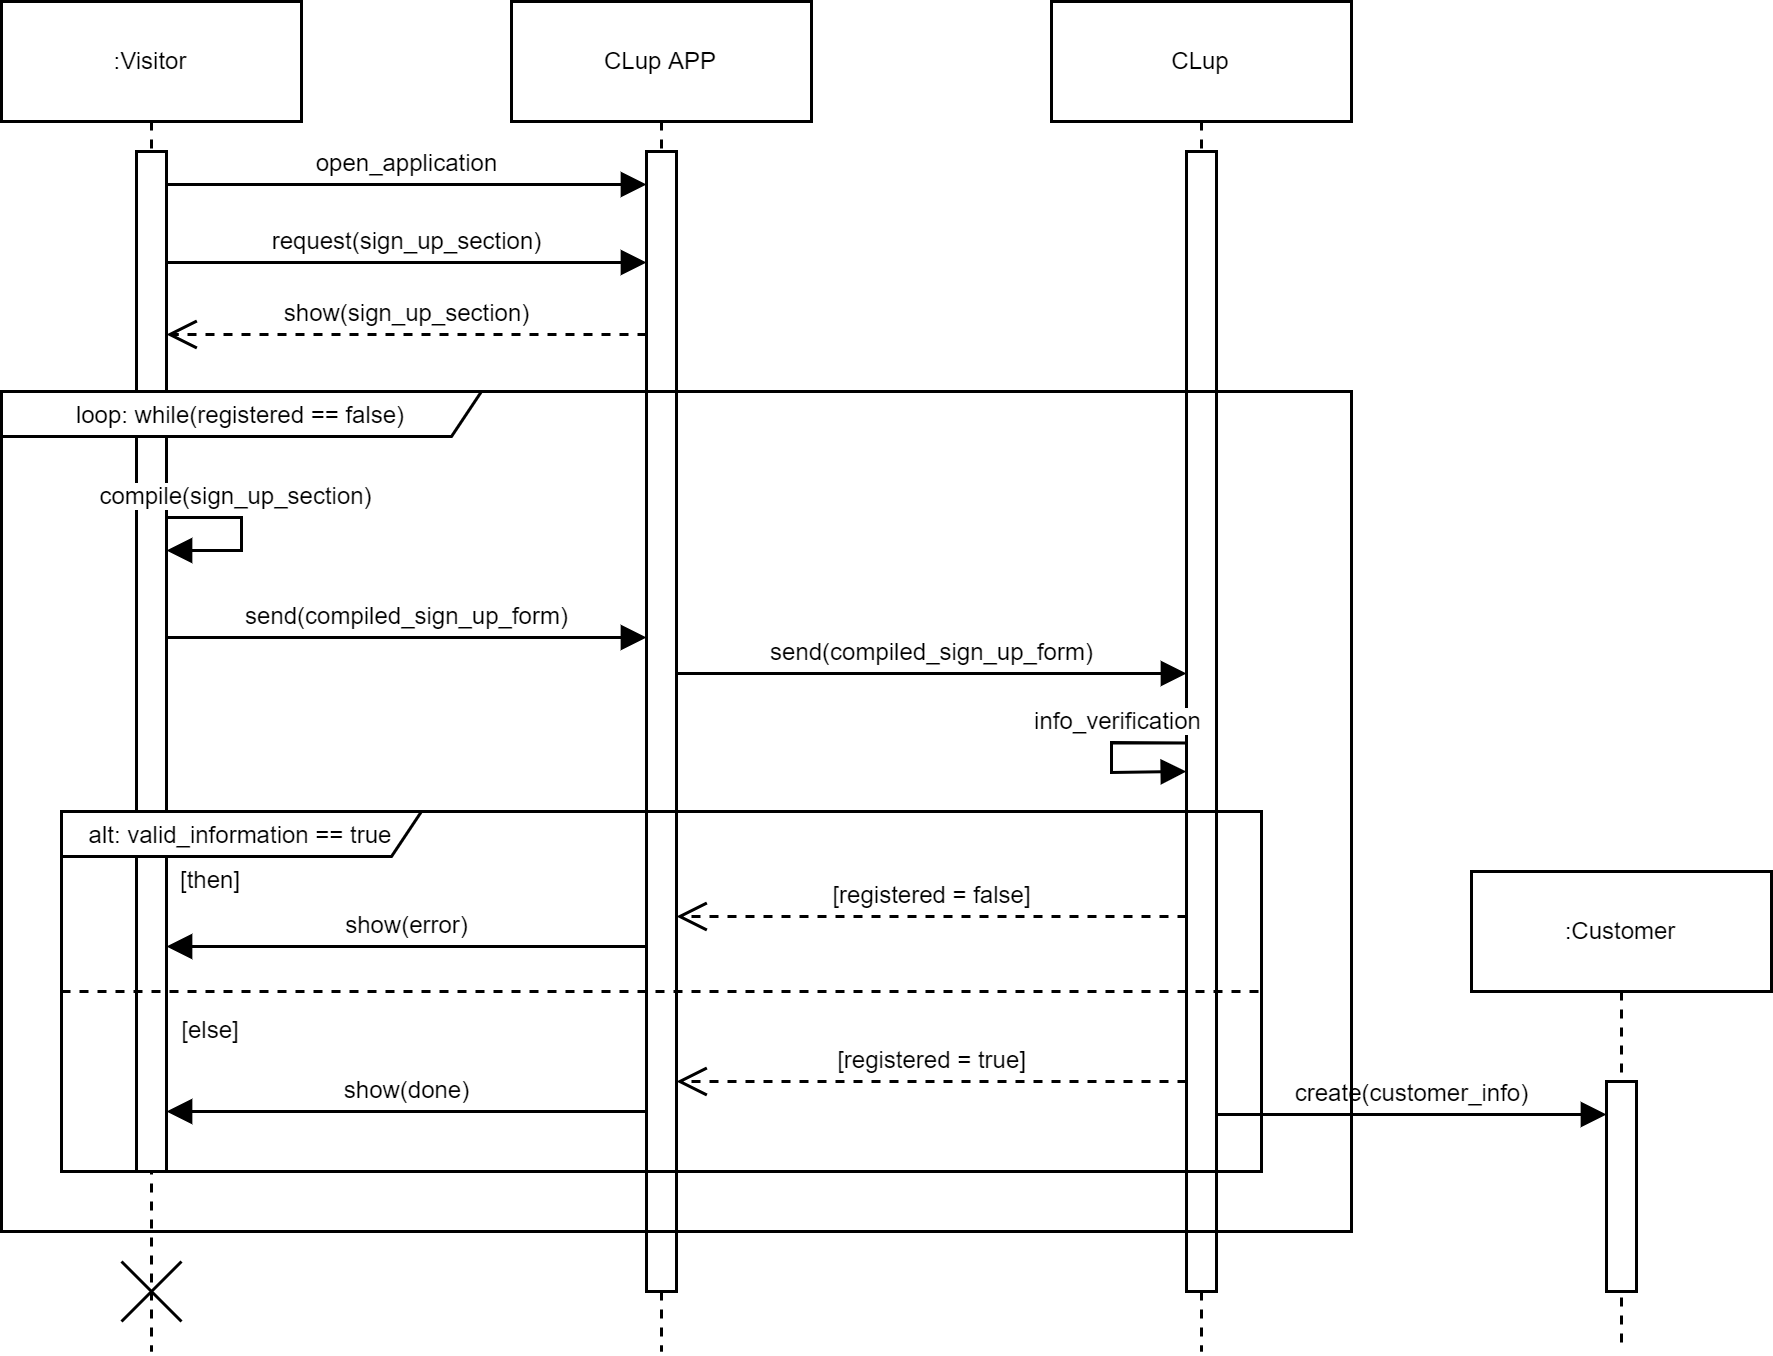
\includegraphics[width=\textwidth]{seq_diagr1.png}
    \caption{Registration to CLup as Customer}
\end{figure}

\begin{figure}
    \centering
    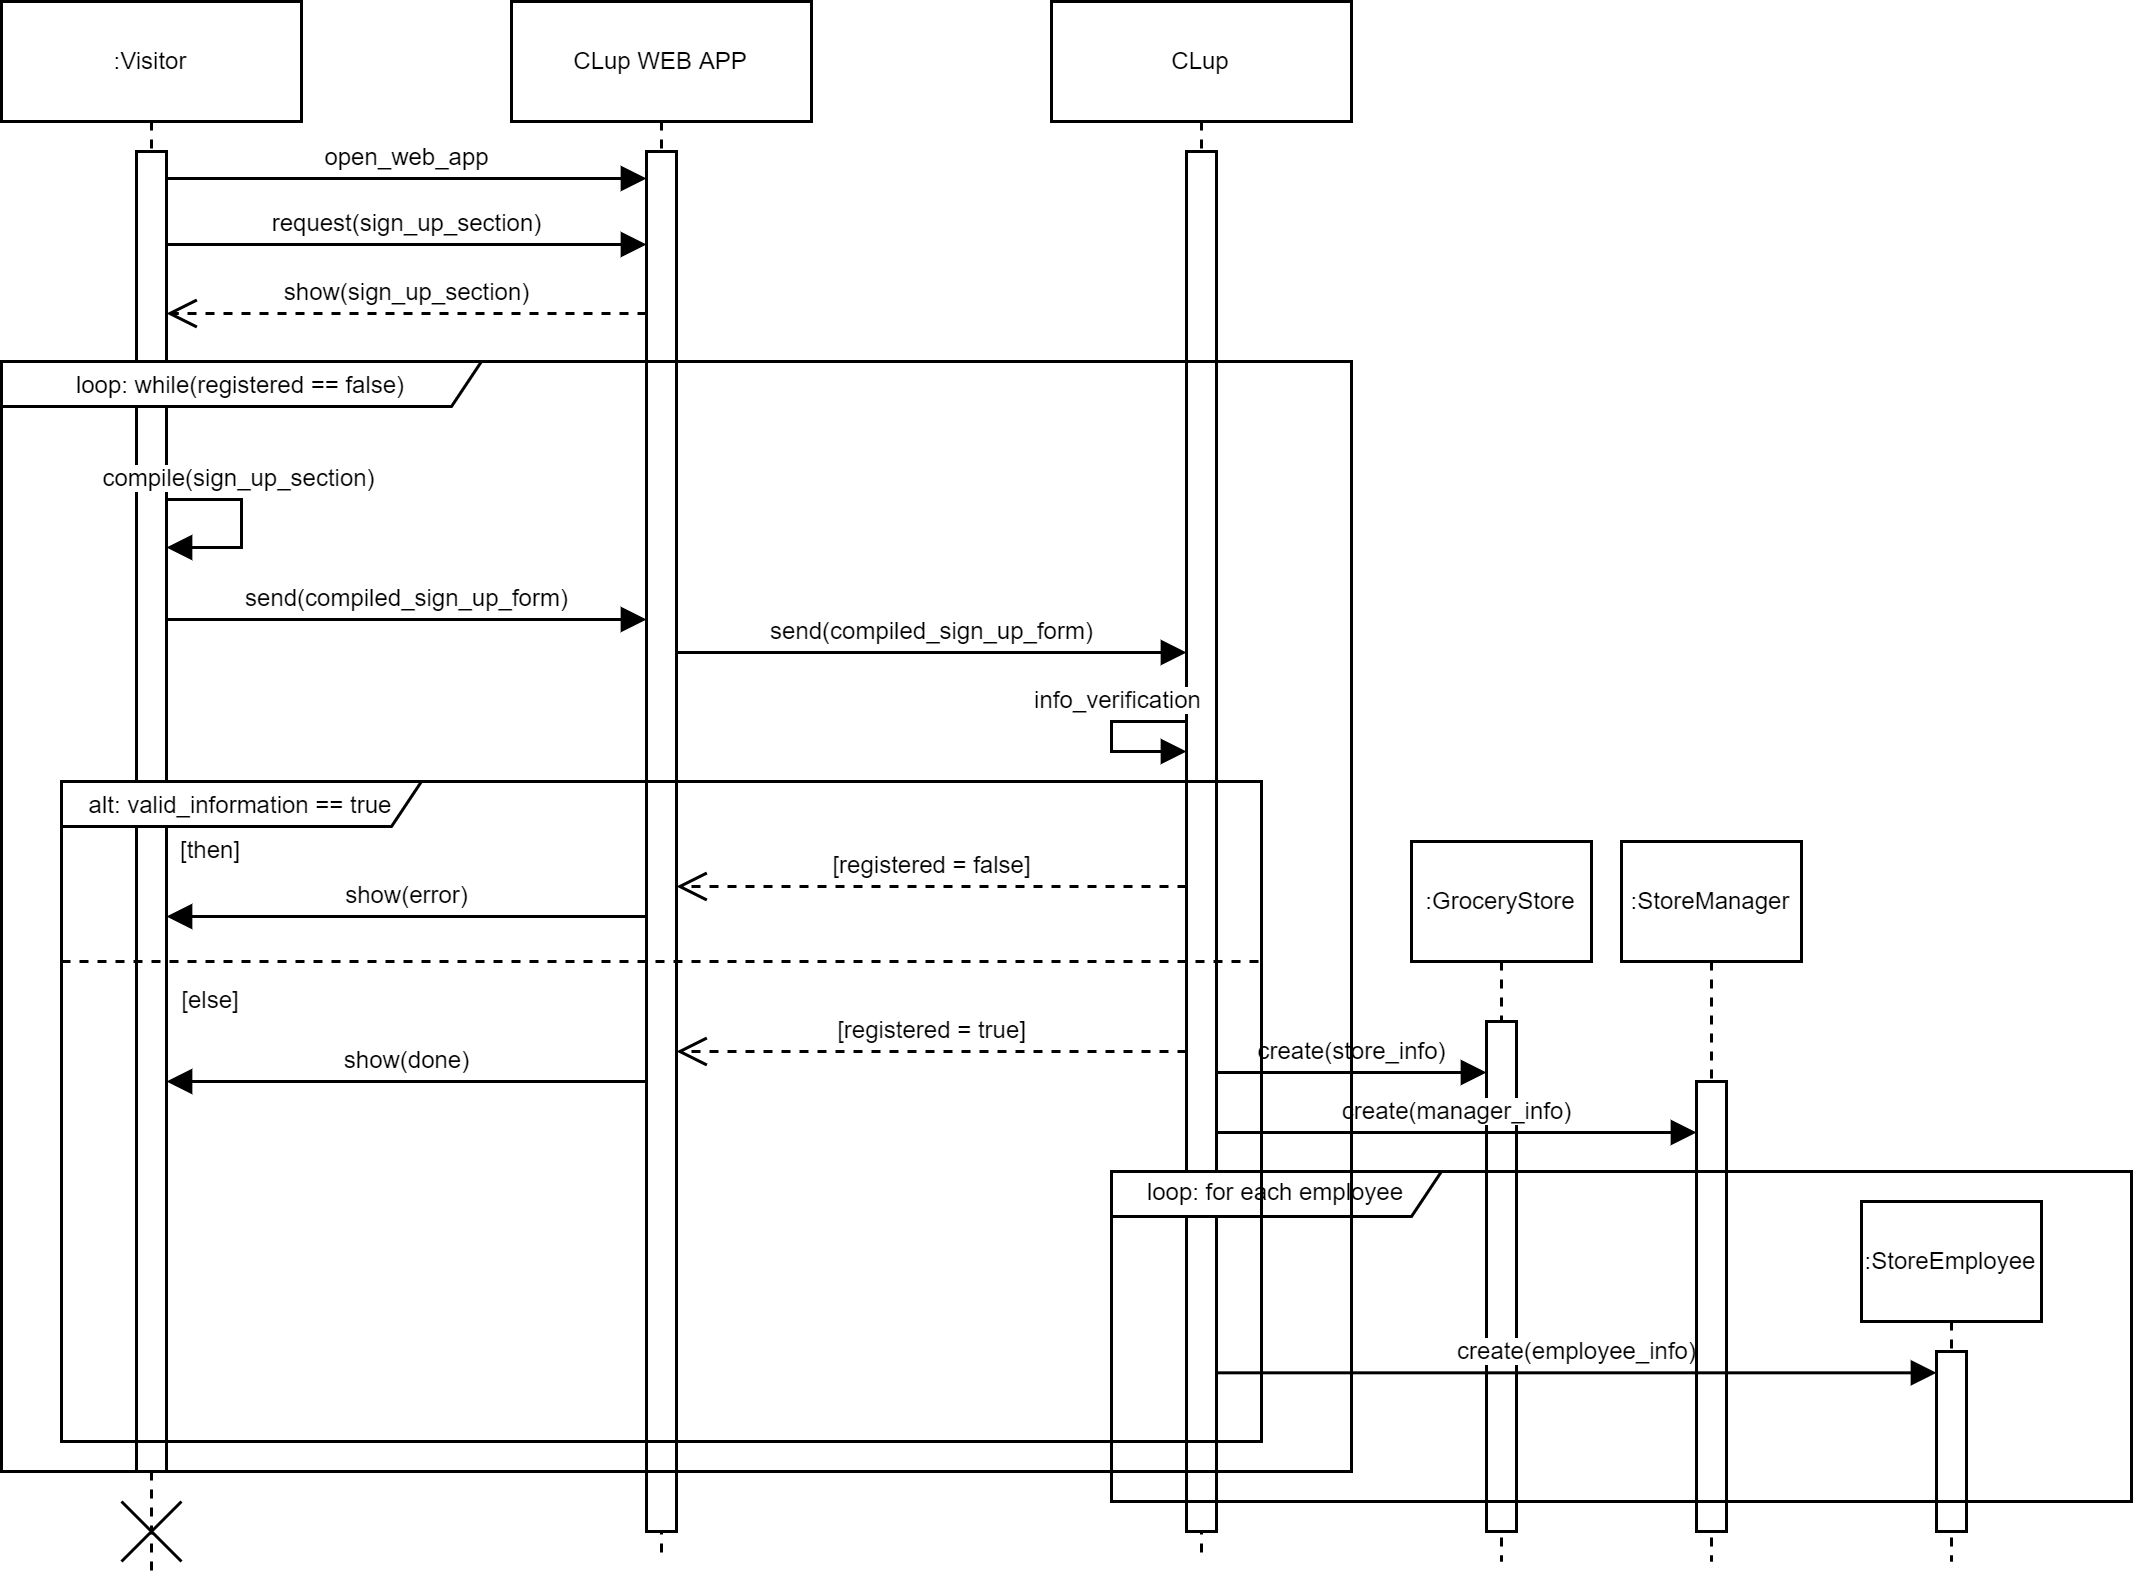
\includegraphics[width=\textwidth]{seq_diagr2.png}
    \caption{Registration to CLup as Store Manager}
\end{figure}

\begin{figure}
    \centering
    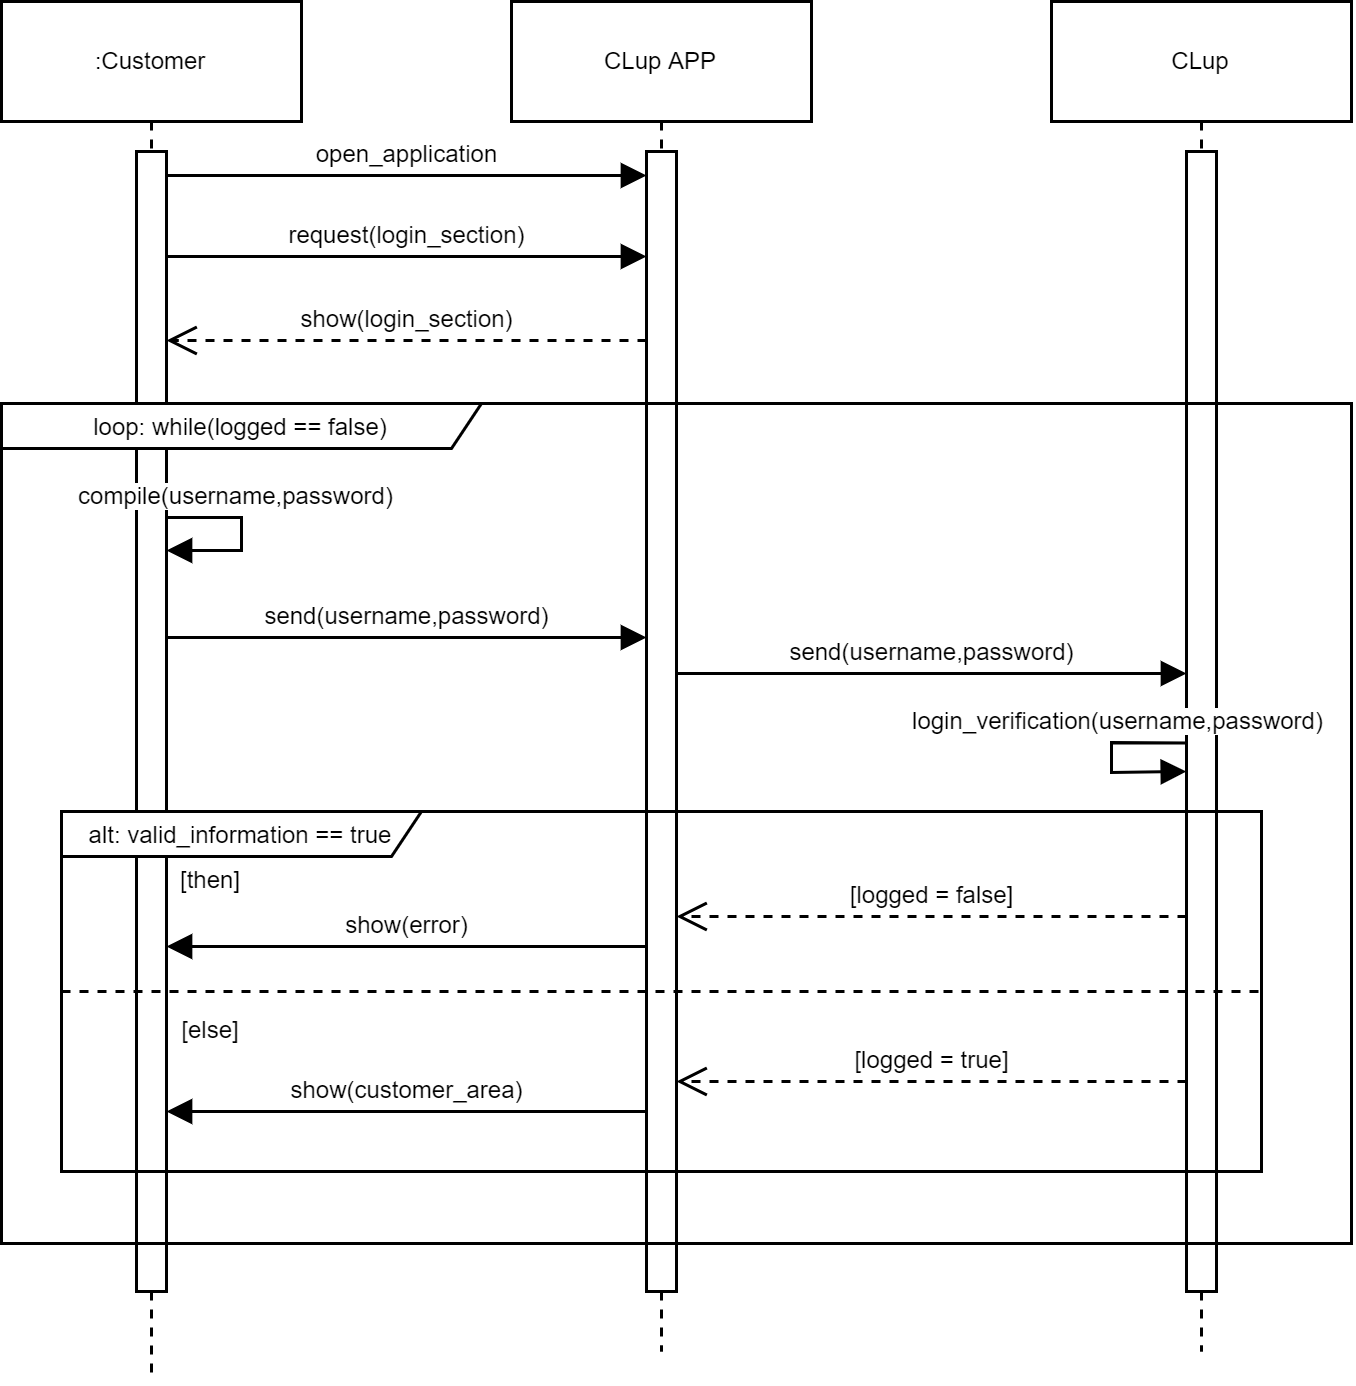
\includegraphics[width=\textwidth]{seq_diagr3.png}
    \caption{Login to the application}
\end{figure}

\begin{figure}
    \centering
    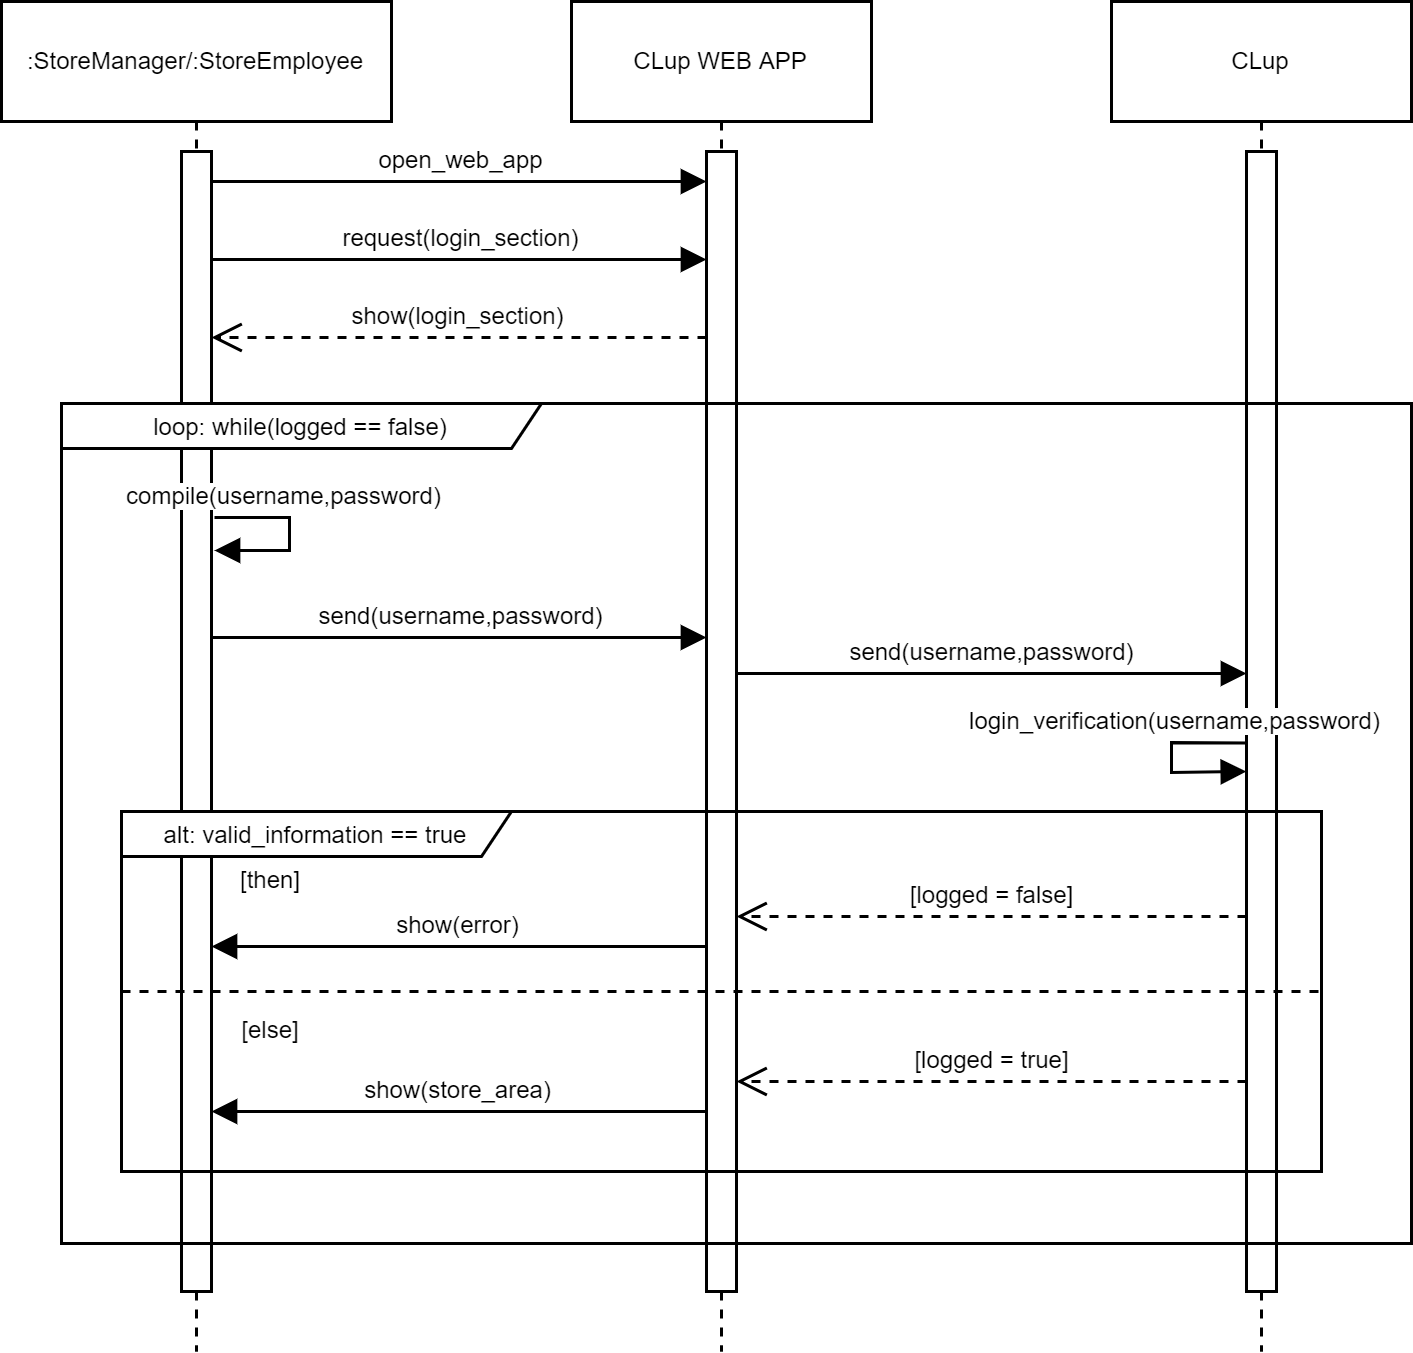
\includegraphics[width=\textwidth]{seq_diagr4.png}
    \caption{Login to the web app}
\end{figure}

\begin{figure}
    \centering
    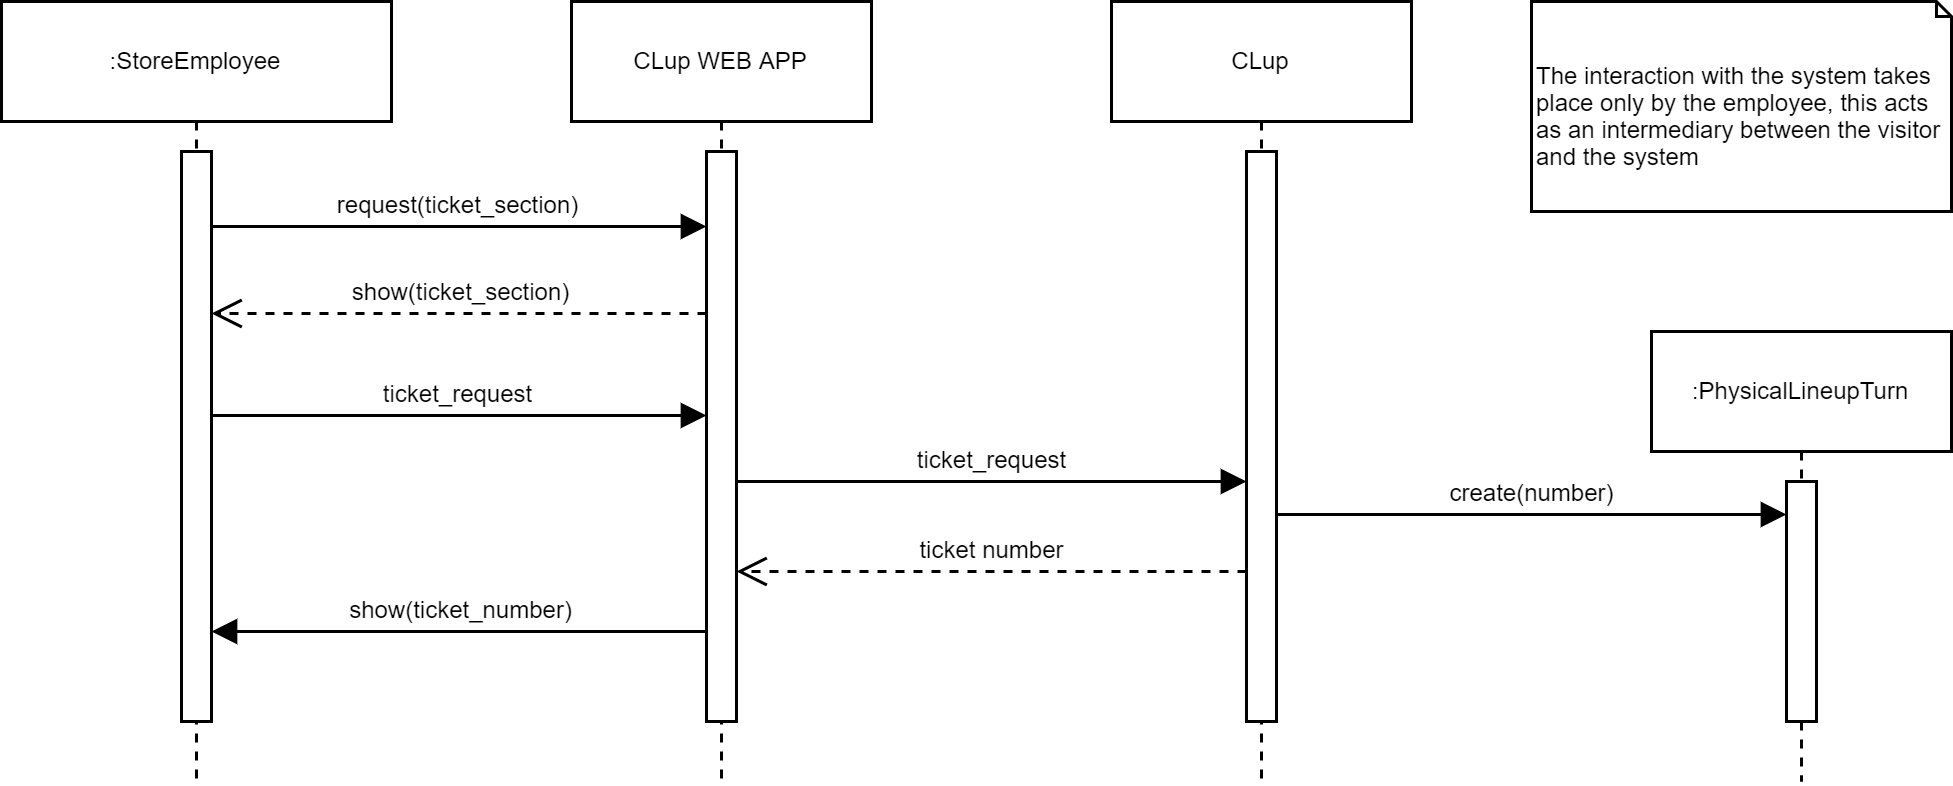
\includegraphics[width=\textwidth]{seq_diagr5.png}
    \caption{Lining up via store}
\end{figure}

\begin{figure}
    \centering
    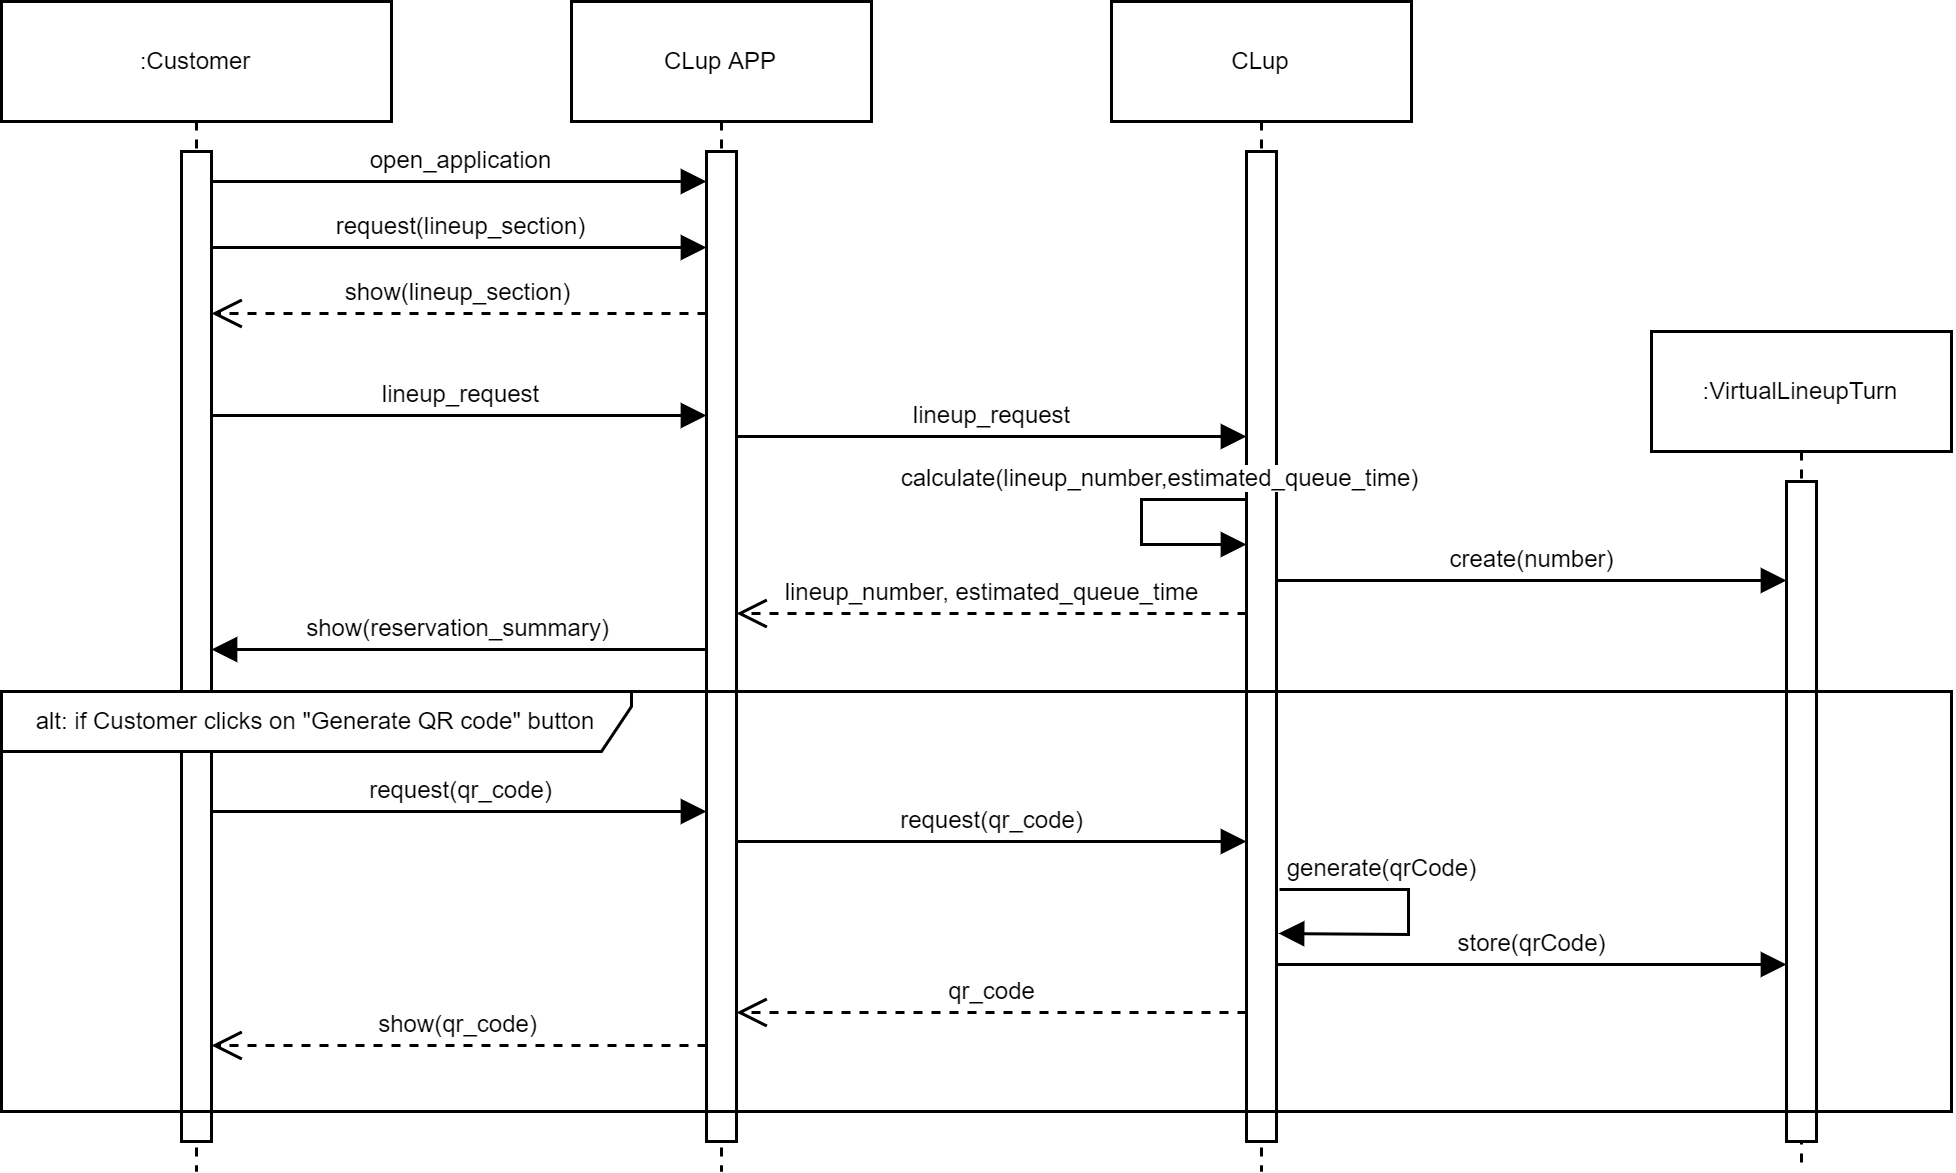
\includegraphics[width=\textwidth]{seq_diagr6.png}
    \caption{Lining up via app}
\end{figure}

\begin{figure}
    \centering
    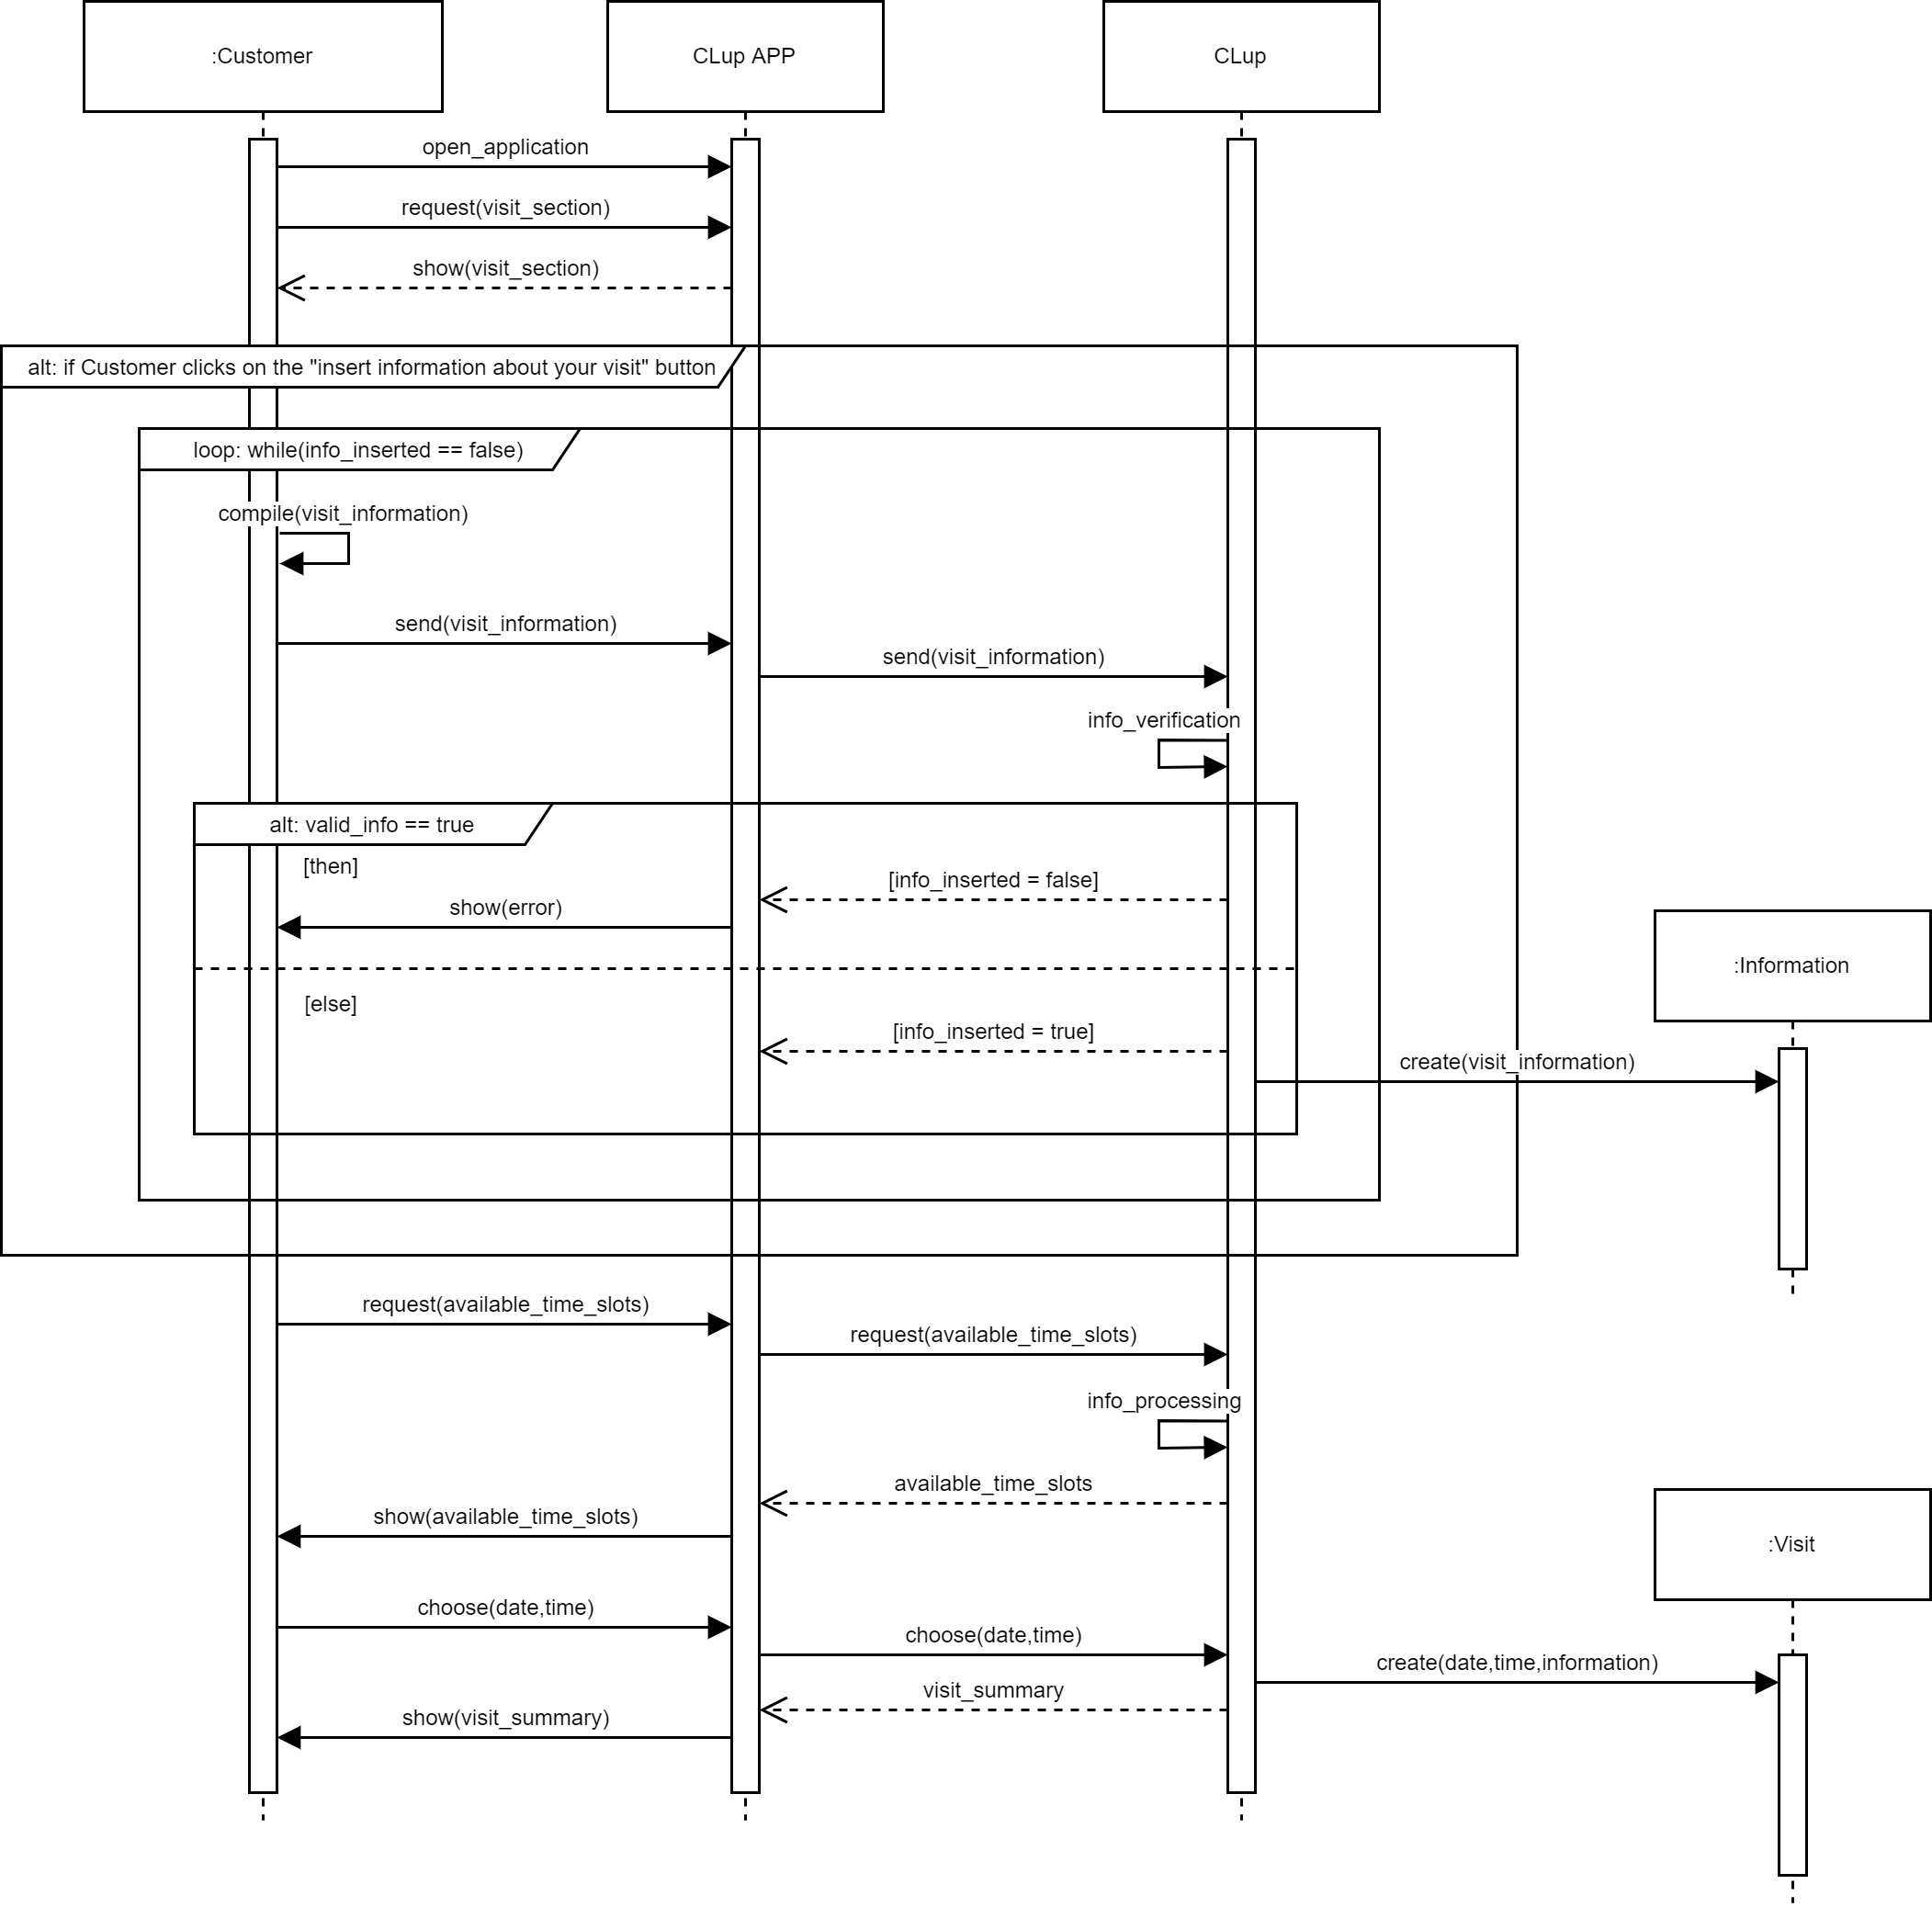
\includegraphics[width=\textwidth]{seq_diagr7.png}
    \caption{Book a visit}
\end{figure}

\begin{figure}
    \centering
    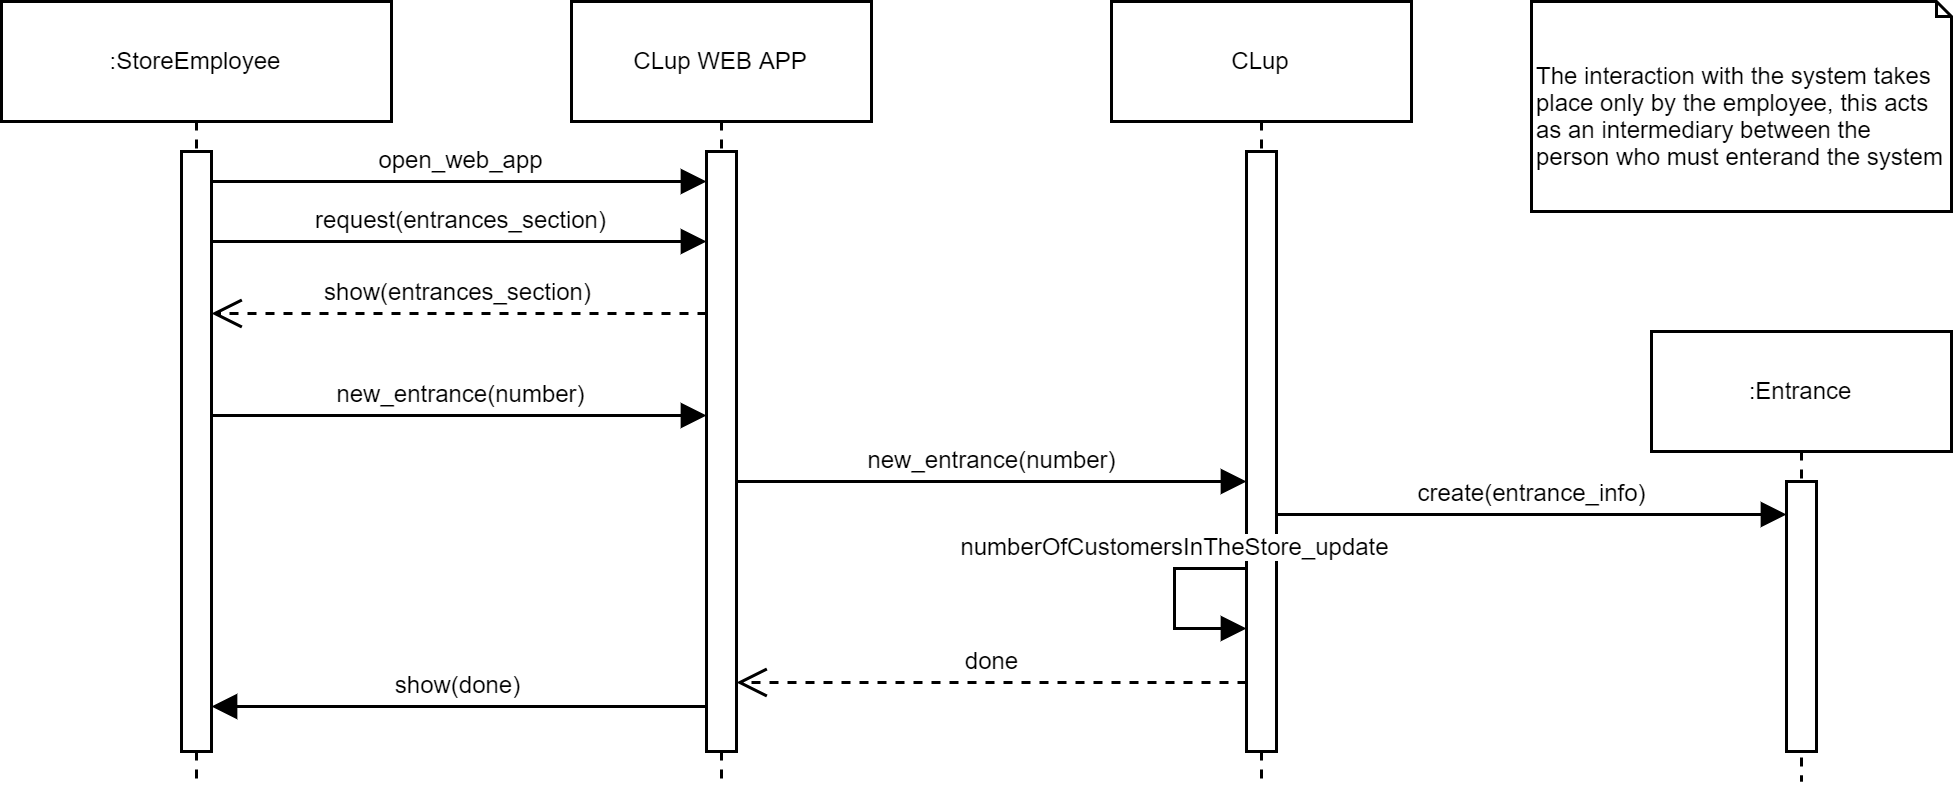
\includegraphics[width=\textwidth]{seq_diagr8.png}
    \caption{Enter the store without QR code after lineup reservation}
\end{figure}

\begin{figure}
    \centering
    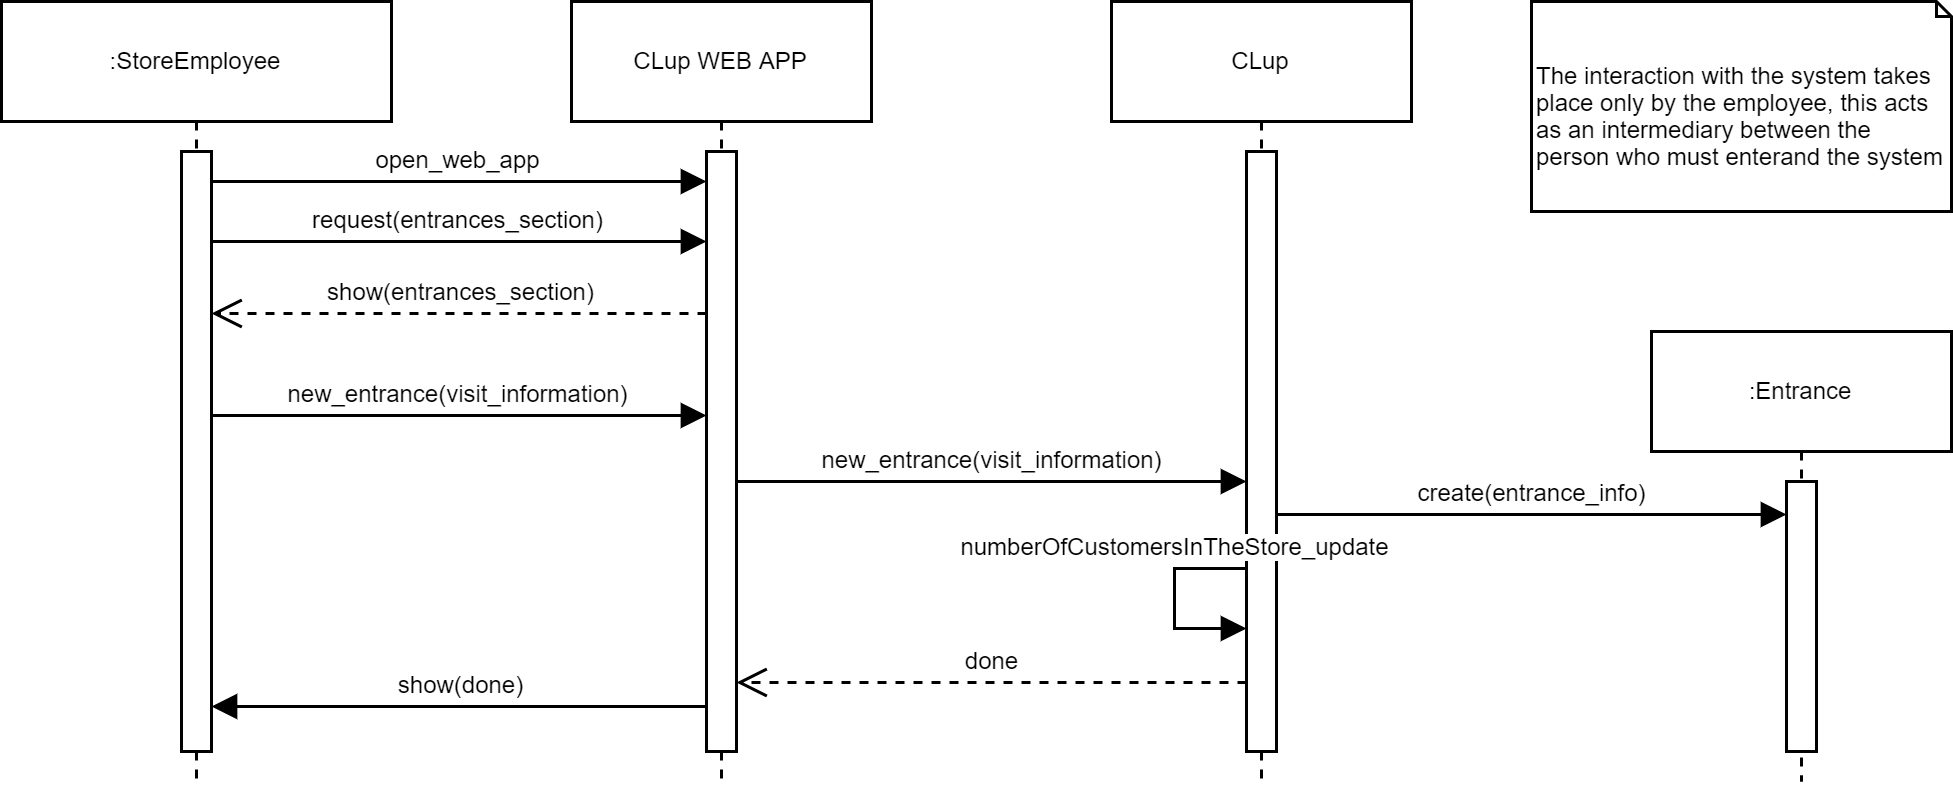
\includegraphics[width=\textwidth]{seq_diagr9.png}
    \caption{Enter the store without QR code for a visit}
\end{figure}

\begin{figure}
    \centering
    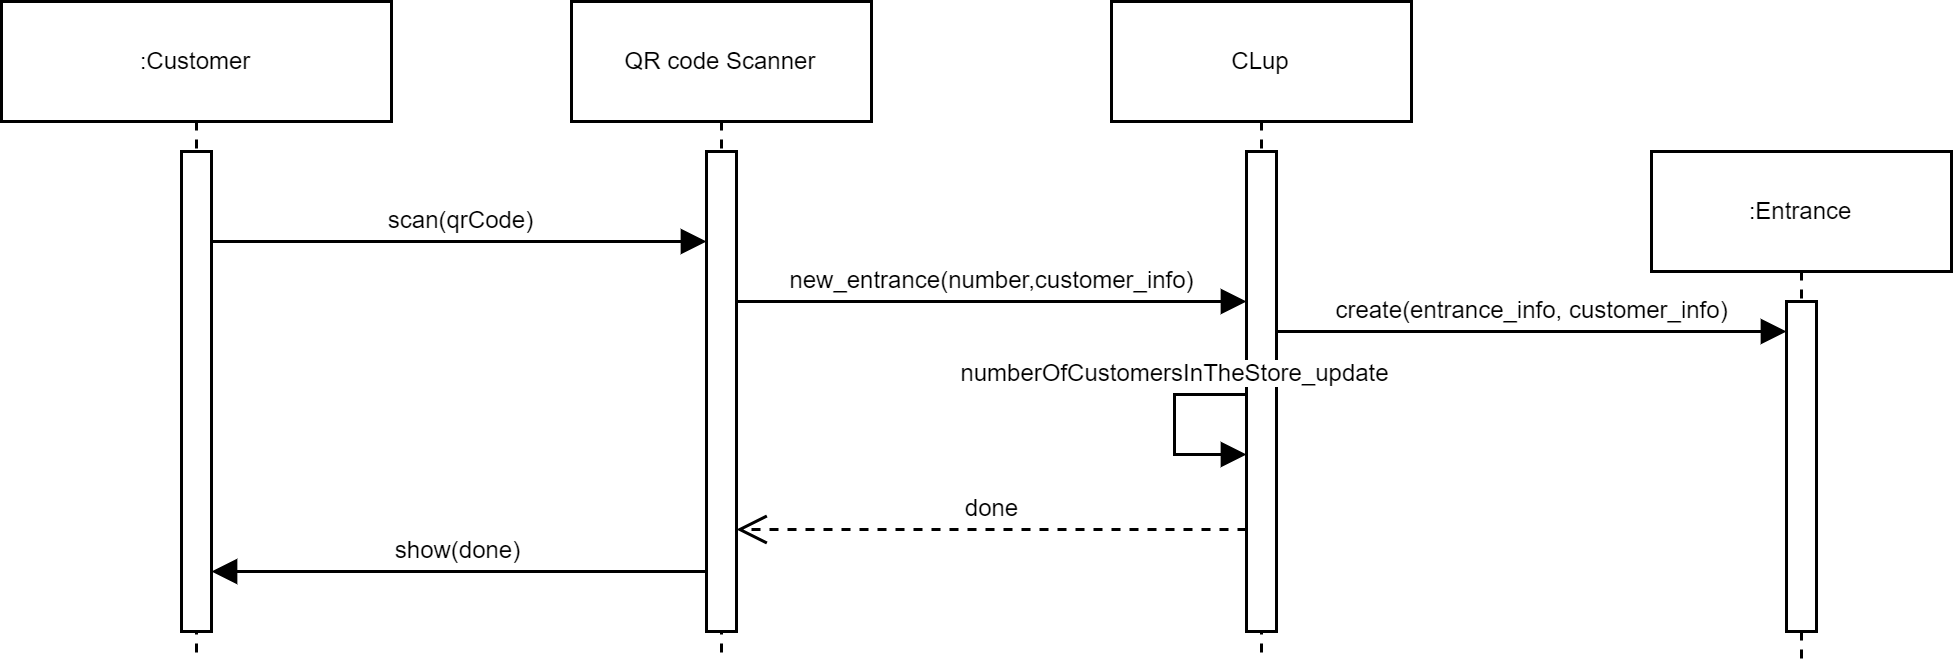
\includegraphics[width=\textwidth]{seq_diagr10.png}
    \caption{Enter the store with a QR code}
\end{figure}

\begin{figure}
    \centering
    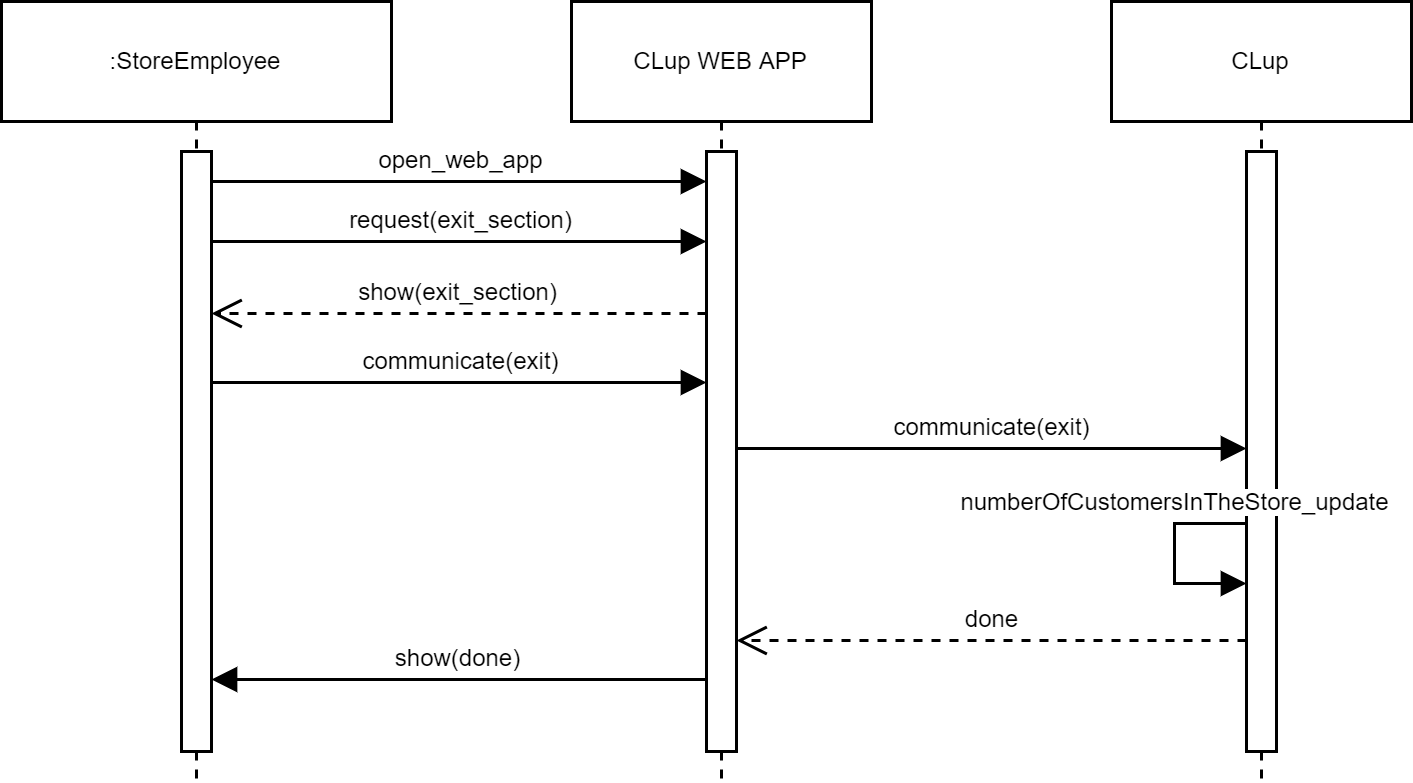
\includegraphics[width=\textwidth]{seq_diagr11.png}
    \caption{Register exit from store}
\end{figure}

\begin{figure}
    \centering
    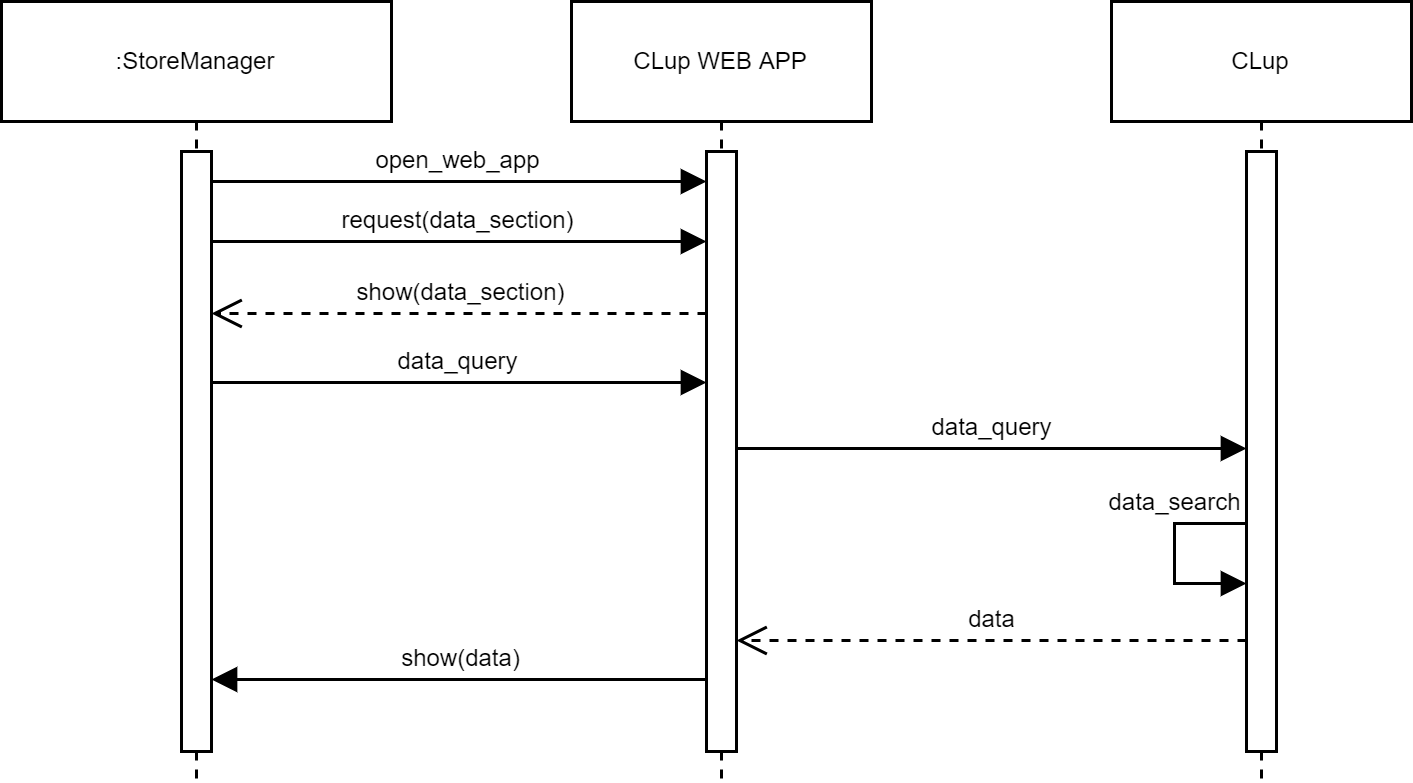
\includegraphics[width=\textwidth]{seq_diagr12.png}
    \caption{Display data of the accesses made through QR code}
\end{figure}

\clearpage

	\section{Performance Requirements}

		The system has to be able to serve a great number of users simultaneously. It has to provide a slow response time to requests. In particular the application and the web application must react in the order of hundreds of milliseconds, except in the case of connectivity issues which must be correctly detected and handled.

	\section{Design Constraints}

		\subsection{Standards compliance}
With regard to the privacy of data the CLup project is subjected to the General Data Protection Regulation (GDPR), a regulation in EU law on data protection and privacy for all individuals within the European Union (EU) and the European Economic Area (EEA).

There are no specific units of measure to adopt. The system has to adopt the international standards about date and time use and representation.

\subsection{Hardware limitations}
As specified in the Hardware limitations (\ref{hardware limitations}) and Hardware Interfaces (\ref{hardware interfaces}) sections are described in detail the hardware specifications. In the following is reported a short summary of all the hardware requirements:
\begin{itemize}
    \item Regarding the customer: Internet connection (2G/3G/4G/Wi-Fi), iOS/Android smartphone and a GPS sensor
    \item Regarding the store manager and the employees: Internet connection (2G/3G/4G/Wi-Fi), modern web browser
\end{itemize}

\subsection{Any other contraint}
Since everyone needs to go to the supermarket the application and the web application should be easy to use and provide intuitive ways to interact with them.

	\section{Software System Attributes}

		\subsection{Reliability}
The system has to be able to run continuosly without any interruptions for long periods of time. To be fault tolerant the system backend deployment must take advantage of some sort of replication and redundancy. The system must have offline backups of the data storage to exploit in a disaster recovery after a data loss.

\subsection{Availability}
Given the fact that CLup is not an emergency service or anything related to critical situations the system must provide an availability of 99.9\%. This means that the average time between the occurence of a fault and service recovery (MTTR) has to be contained at around 0.365 days per year. 

\subsection{Security}
The data provided by the users contain some sensitive informations, so the security aspect cannot be underestimated. The central database must be protected with all the available measures to avoid any external or internal attack. The passwords inside the data store has to be encrypted and in case of password recovery this must never be sent in clear.

To communicate over the internet CLup must use some sort of encryption to avoid traffic sniffing and spoofing, thus avoiding cheating attacks and guaranteeing privacy and consistency.

\subsection{Maintanability}
The system must guarantee a high level of maintainability. Appropriate design patterns should be used, toghether with good standards. The code must be well documented and hard-coding must be avoided. A testing routine has to be provided and it has to cover at least 75\% of the entire codebase, excluding interfaces code.

\subsection{Portability}
The application must be developed for two different platforms: iOS and Android smartphones. The web application must run on any OS (like Windows, Mac OS, Linux, ecc) that supports a web browser. Even mobile devices like iPads and Android tablets must be able to access the web app.

\chapter{Formal Analysis Using Alloy}\label{chapt:sum}

\chapter{Effort Spent}\label{chapt:sum}

\chapter{References}\label{chapt:sum}

\pagebreak


% Adding a bibliography if citations are used in the report
\bibliographystyle{plain}
\bibliography{BiBTeXexempel.bib}
% Adds reference to the Bibliography in the ToC
\addcontentsline{toc}{chapter}{\bibname}

\end{document}